% !TEX root = mythesis.tex

%==============================================================================
\chapter{The Pierre Auger Observatory}
\label{chap:setup}
%==============================================================================
\begin{figure}[h!]
\centering
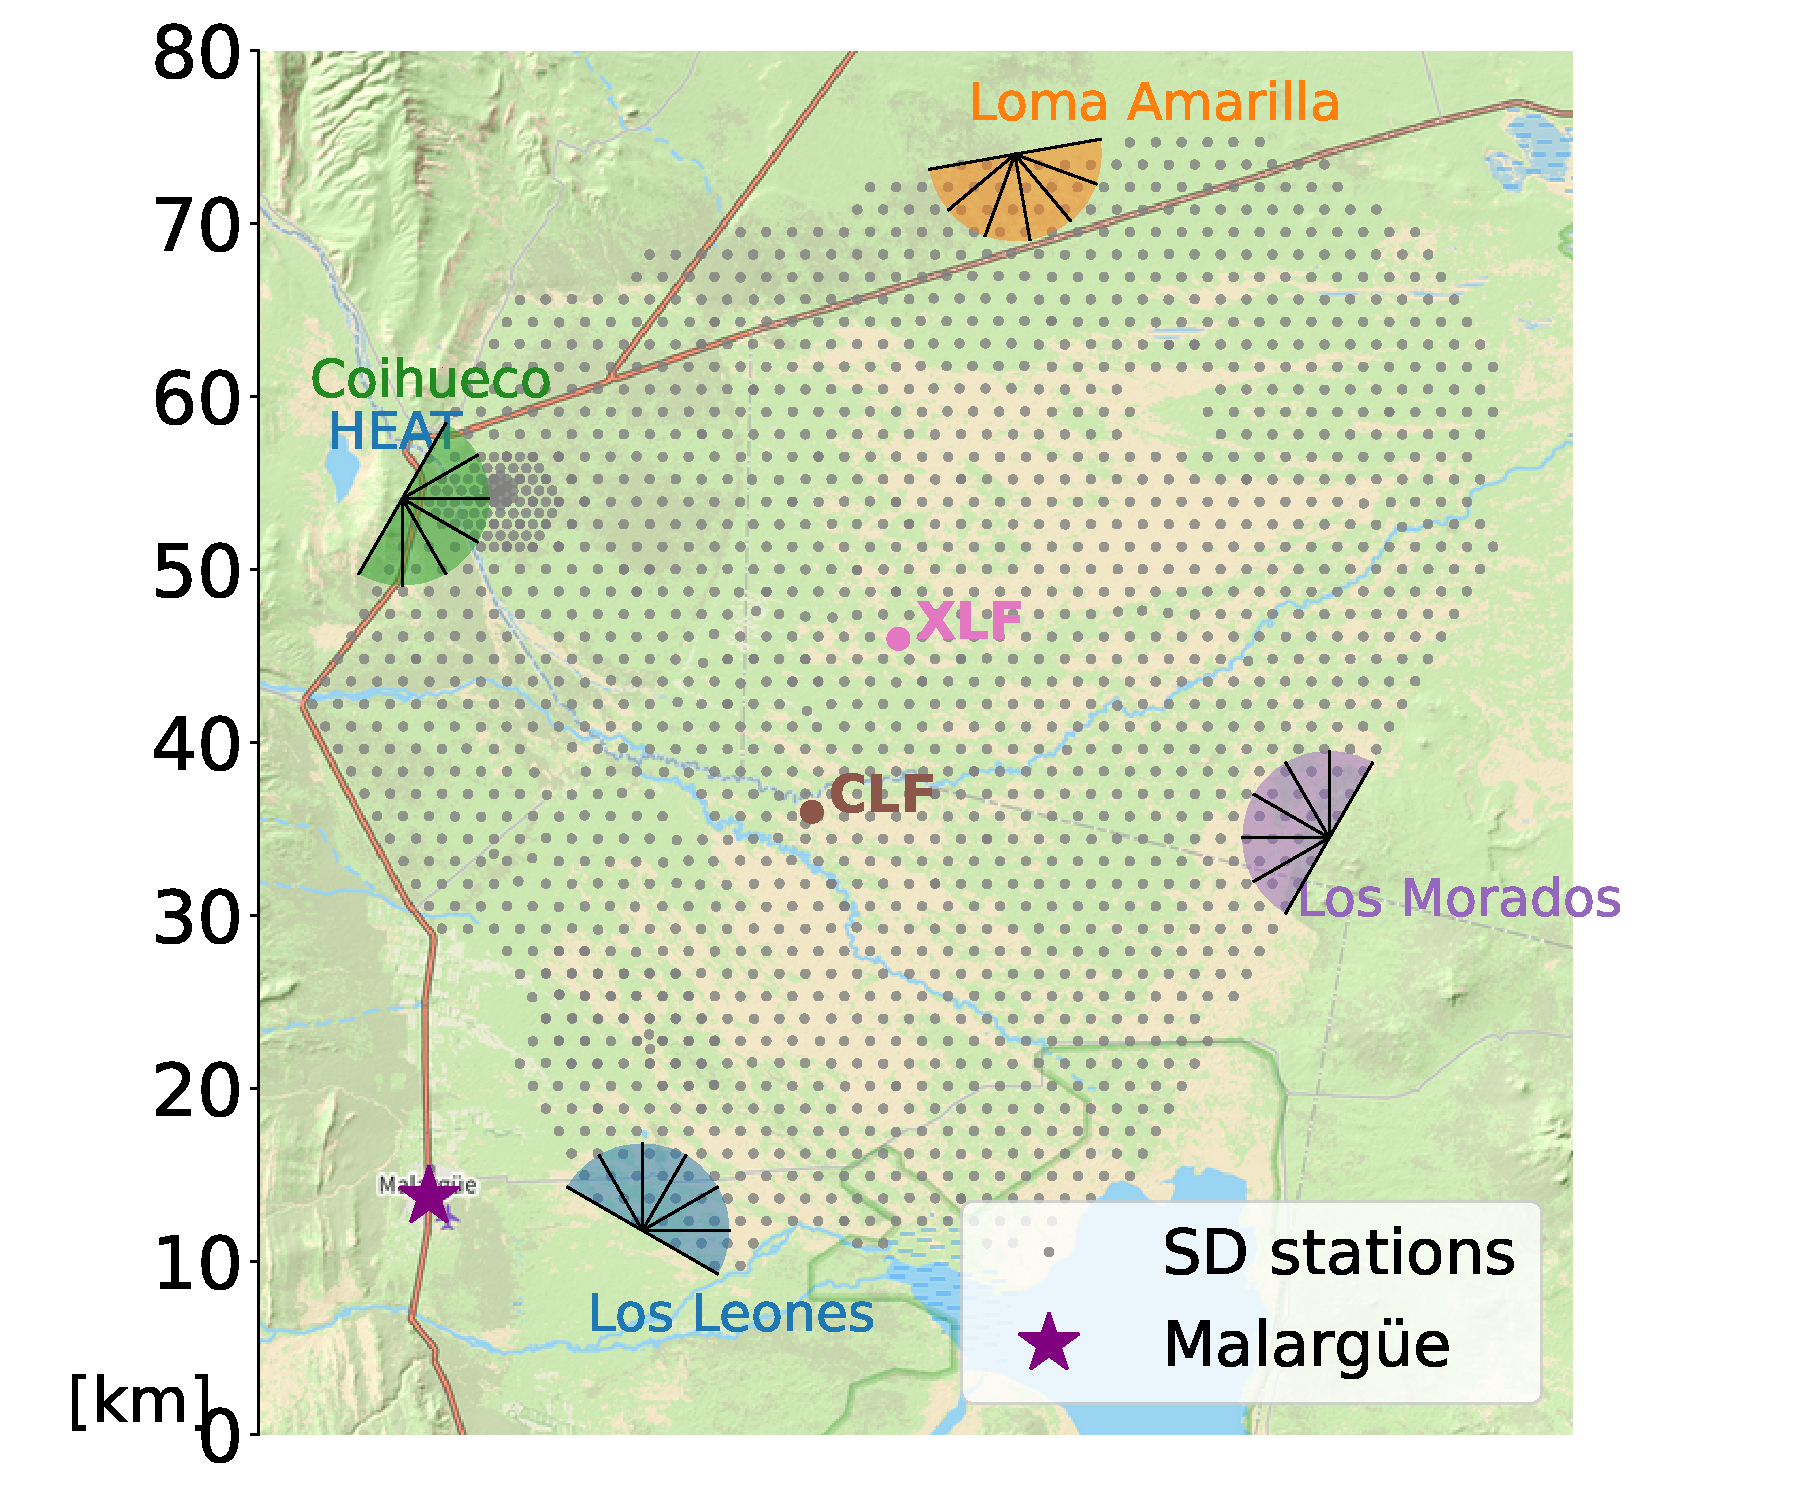
\includegraphics[width=\textwidth]{thesis_figures/Setup/map_srij_version.pdf}
\caption{Layout of the Pierre Auger Observatory in Argentina. The black lines indicate the field of view of each telescope. Redone from~\cite{Jannis_thesis} }
\label{fig:Auger_map}
\end{figure}

The Pierre Auger Observatory~\cite{Auger:2015} is the largest CR observatory in the world. Located outside Malargüe in the Argentinian \textit{pampas}, the observatory spans across an area of 3000 km$^2$. Originally conceptualized in the 1990s, it was built in the early 2000s and fully completed in 2008. Geographically the site is located near the base of the Andes at an altitude of 1400 m above sea level and is relatively flat across its whole span. The observatory was designed to detect CR-induced EASs having primary energy of $10^{17}$eV to $10^{20}$eV and beyond. It does so by identifying the EAS via two different complementary detecting components: \textit{\acrlong{SD}} array (\acrshort{SD}) and the \textit{Fluorescence Detector} (\acrshort*{FD}). A schematic of the observatory is shown in Fig.~\ref{fig:Auger_map}. The SD consists of 1660 water Cherenkov tanks spread in a triangular grid with 1.5 km spacing. The FD consists of four sites with 27 telescopes located at the edges of the ground array and overlooking the sky above. The observatory also consists of various atmospheric monitoring devices such as LIDARs~\cite{BENZVI2007171}, laser facilities~\cite{article_clf,Lawrence_Wiencke_2009} and other weather sensors to constantly monitor the atmosphere which is important for FD operation. With the AugerPrime upgrade of the observatory which is scheduled to be finished in 2024 two new detecting components are being added: The \textit{\acrlong{RD}} (\acrshort{RD})~\cite{Horandel:2023XL} and the \textit{\acrlong{UMD}} (\acrshort{UMD})~\cite{AbdulHalim:2023ZF}. The tanks are also being upgraded with the addition of a scintillator on top~\cite{Cataldi:2021uwd}. The individual components of the new upgrade are not discussed in detail since they are not used in the context of this thesis but only AugerPrime as a whole and its potential for detecting neutrinos at the Pierre Auger Observatory is discussed later.

Even though, the primary objective of the Pierre Auger Observatory is UHECR physics it is also sensitive to the neutrino induced EAS signature via both the SD and FD. The low neutrino interaction probability requires a detector that is always active. The high duty cycle of the SD $\simeq 100$\% compared to a limited duty cycle of the FD $\simeq 15$\% makes SD the more probable of the detector to detect neutrinos. This has already been shown in previous neutrino searches at Auger where the search with the SD provides the most stringent limits to the diffuse flux of ultra-high-energy neutrinos~\cite{Aab_2019_diffuse}. This chapter aims to provide a short review of the different components of the observatory with a focus on the SD and its trigger system since it is the primary detector used for the analysis presented in this thesis. 

\section{Fluorescence Detector}
\label{sec:Fl_det}
The Fluorescence Detector system at the Pierre Auger Observatory consists of an array of Fluorescence telescopes that are constantly looking inwards over the surface detector array trying to measure the nitrogen fluorescence induced by the EAS. The FD consists of 24 telescopes located at four different small hills (Coihueco, Los Morados, Loma Amarilla and Los Leones). The Coihueco site also consists of \gls{HEAT} which can be tilted upwards to extend the field of view at the Coiheuco site. Each of the 24 telescopes has a field of view of $30^{\circ} \times 30^{\circ}$ in azimuth and elevation. The combination of the telescopes gives an azimuth coverage of $180^{\circ}$. The HEAT telescopes can extend the field of view by a further $30^{\circ}$ in elevation. This gives a 100\% triggering efficiency for EAS above $10^{19}$eV for FD and above $10^{17}$eV with the inclusion of HEAT. Currently, the FD is always operated in combination with SD. As mentioned before the measured fluorescence light gives the deposited shower energy which is about 90\% of the total. The remaining 10\% which is carried by non-fluorescence producing particles such as neutrinos and muons is corrected with simulations~\cite{Abraham_2010_FD}. The expected fluorescence yield (combined for all wavelengths) is affected by the temperature, pressure and humidity of air~\cite{Rosado:2014bya}. This is constantly monitored at the observatory via several monitoring instruments. Each FD site is equipped with a LIDAR station which continuously monitors the aerosol profile, cloud and sky cameras which photograph the sky to estimate the cloud coverage and wind and rain sensors for the safe functioning of the FD telescopes. Two laser facilities \gls{CLF} and \gls{XLF} have also been functional since 2003 and 2008 respectively. These help provide hourly measurements of the atmospheric aerosol content and can also be used to measure FD performance. 


% \begin{figure}[t!]
%   \centering
%   \begin{subfigure}[b]{0.45\textwidth}
%       \centering
%       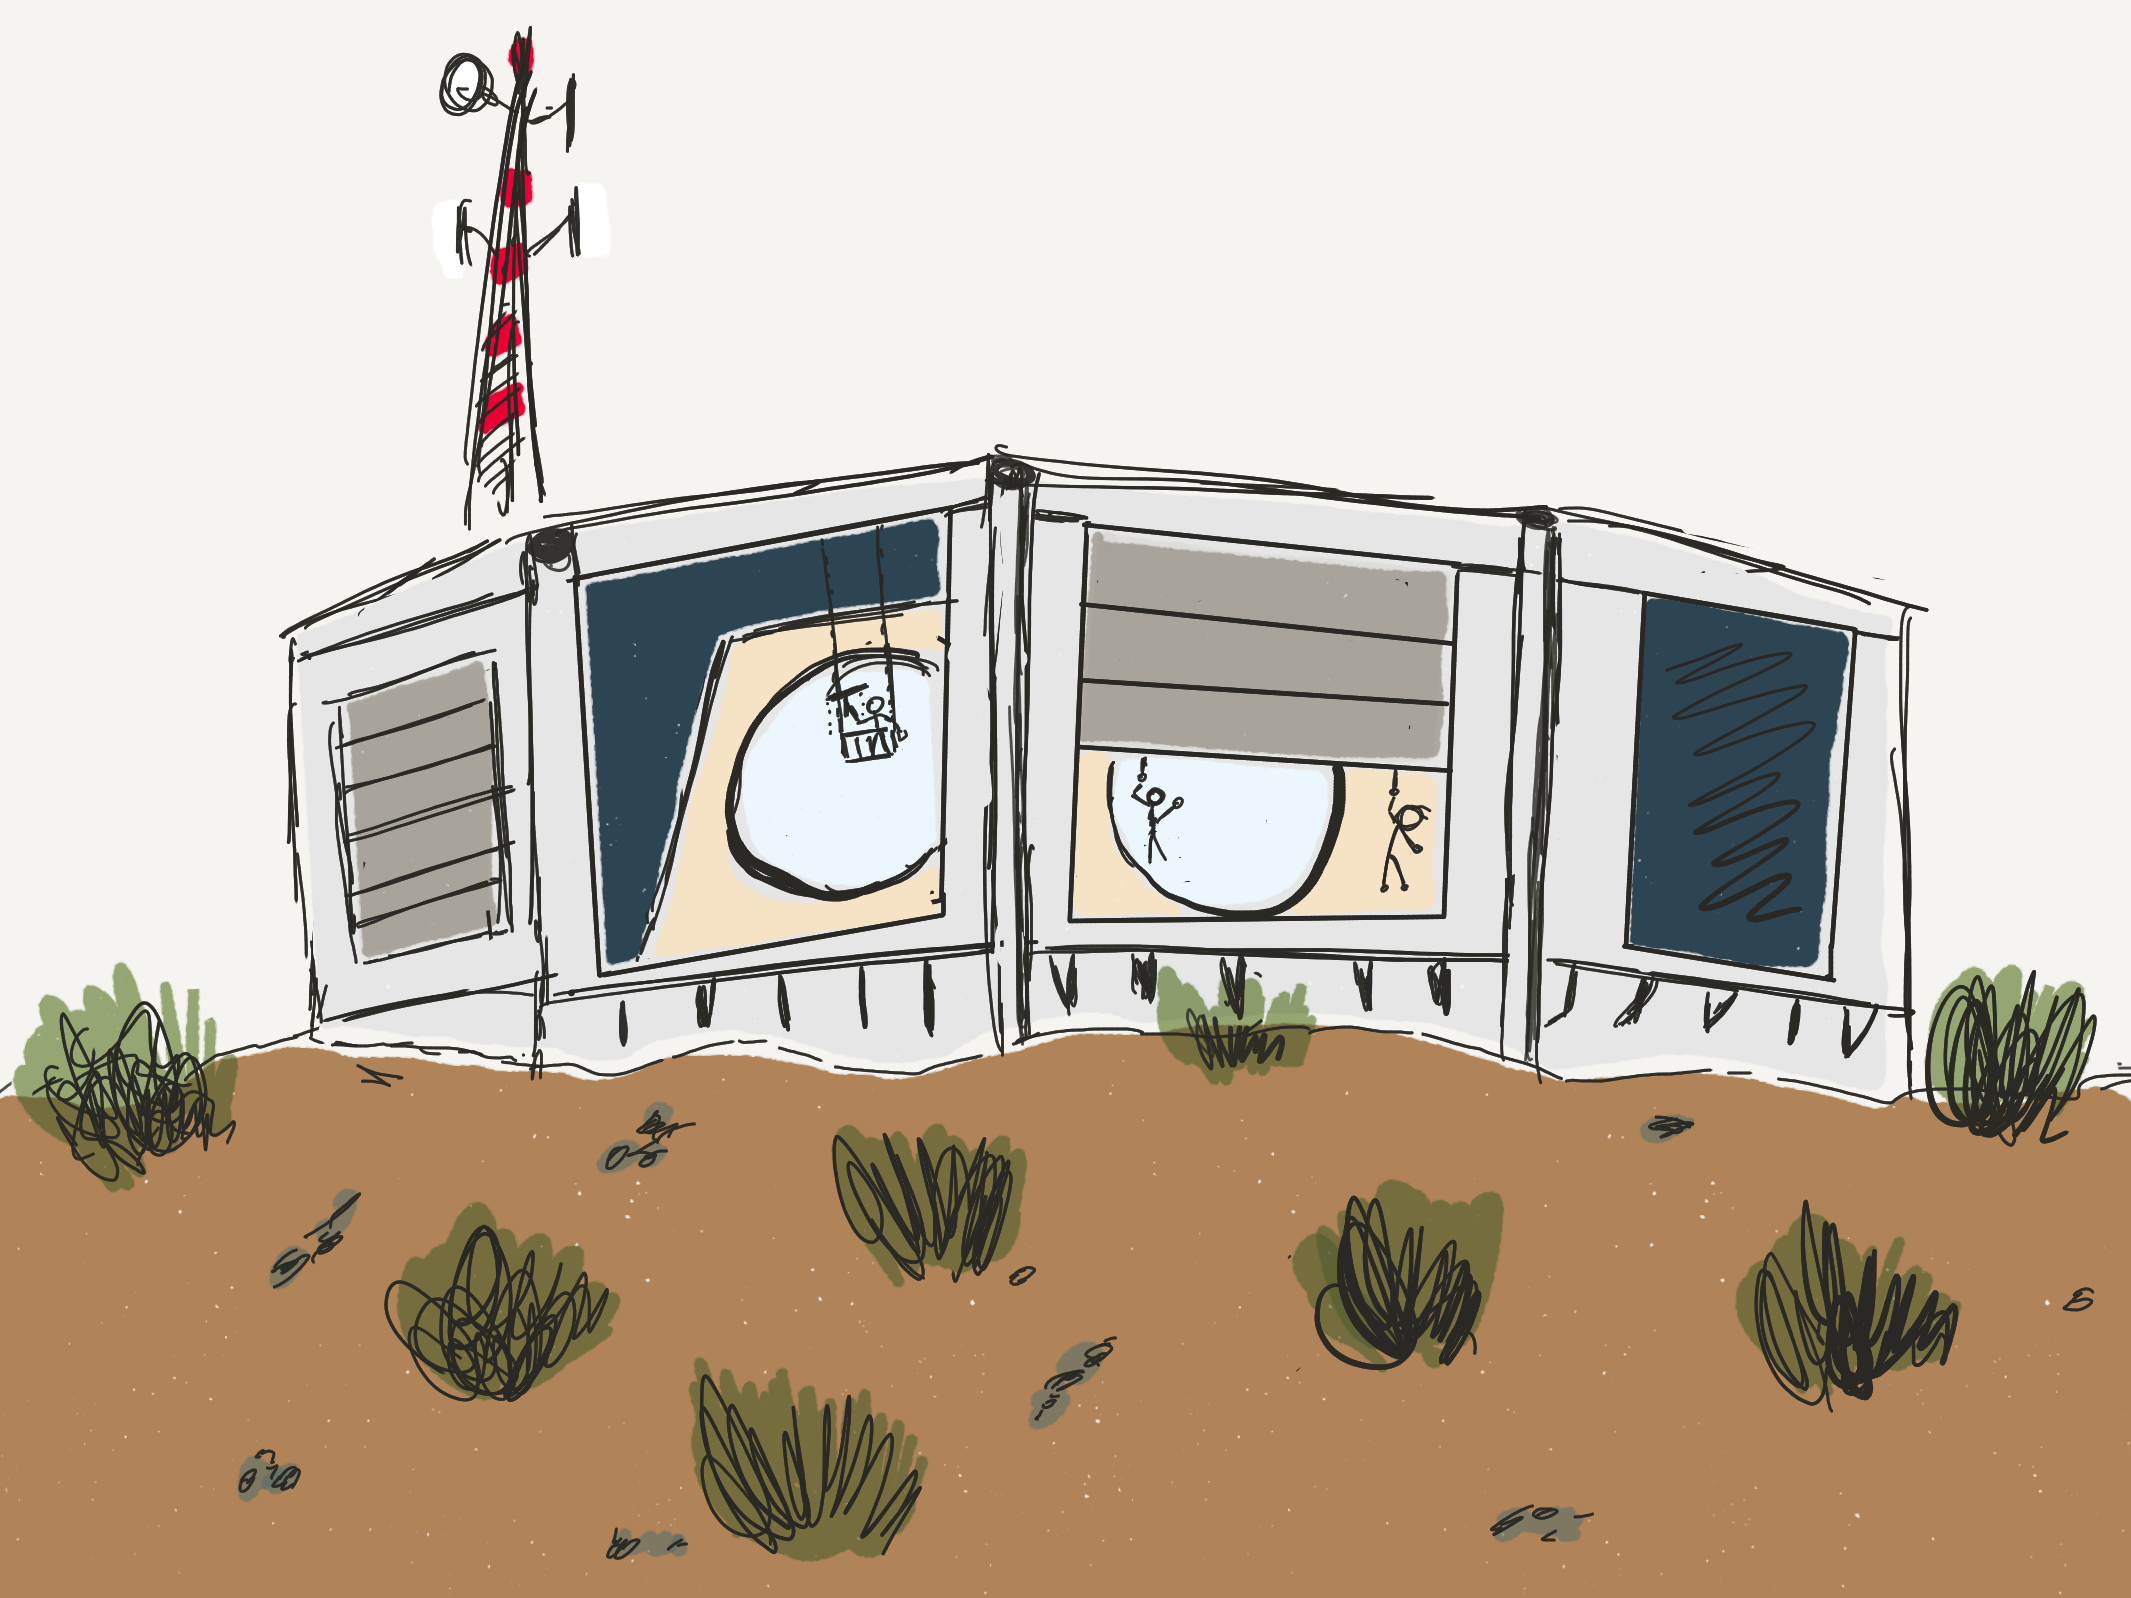
\includegraphics[width=\textwidth]{thesis_figures/Setup/FD_outside_drawing.png}
%       \caption{An artistic drawing inspired by the FD building at Los Leones.}
%       \label{sub:fig:FD_site_drawing}
%   \end{subfigure}
%   \hfill
%   \begin{subfigure}[b]{0.45\textwidth}
%       \centering
%       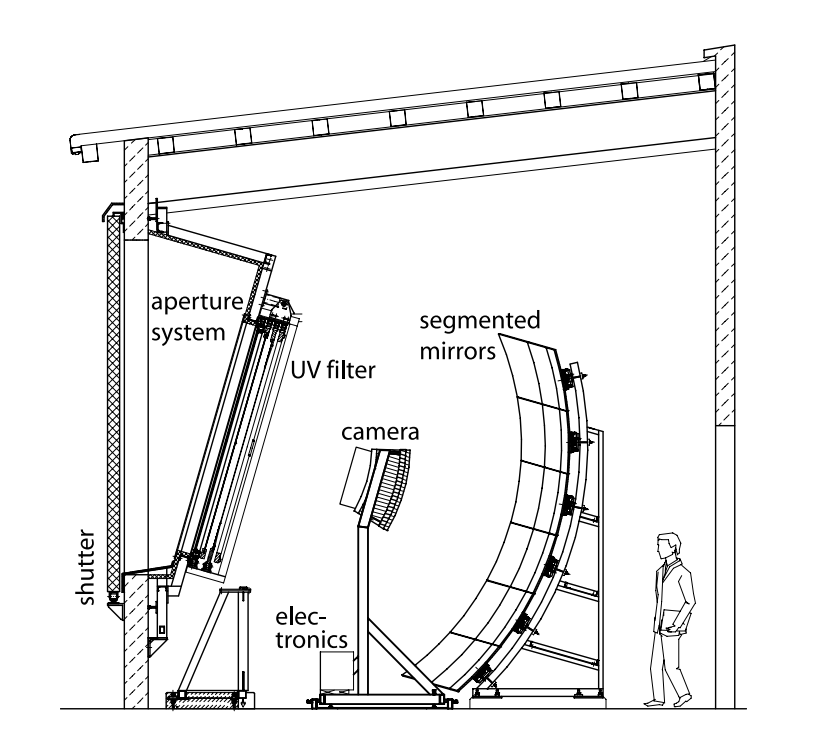
\includegraphics[width=\textwidth]{thesis_figures/Setup/FD_schematic.png}
%       \caption{Schematic view of a fluorescence telescope with a description of its main components taken from~\cite{Auger:2015}}
%       \label{sub:fig:FD_schematic}
%   \end{subfigure}
%      \caption{Fluorescence Telescope at Pierre Auger Observatory}
%      \label{fig:FD_sketch_schematic}
% \end{figure}

\begin{figure}
  \centering
  \subcaptionbox{An artistic drawing inspired by the FD building at Los Leones.\label{sub:fig:FD_site_drawing}}{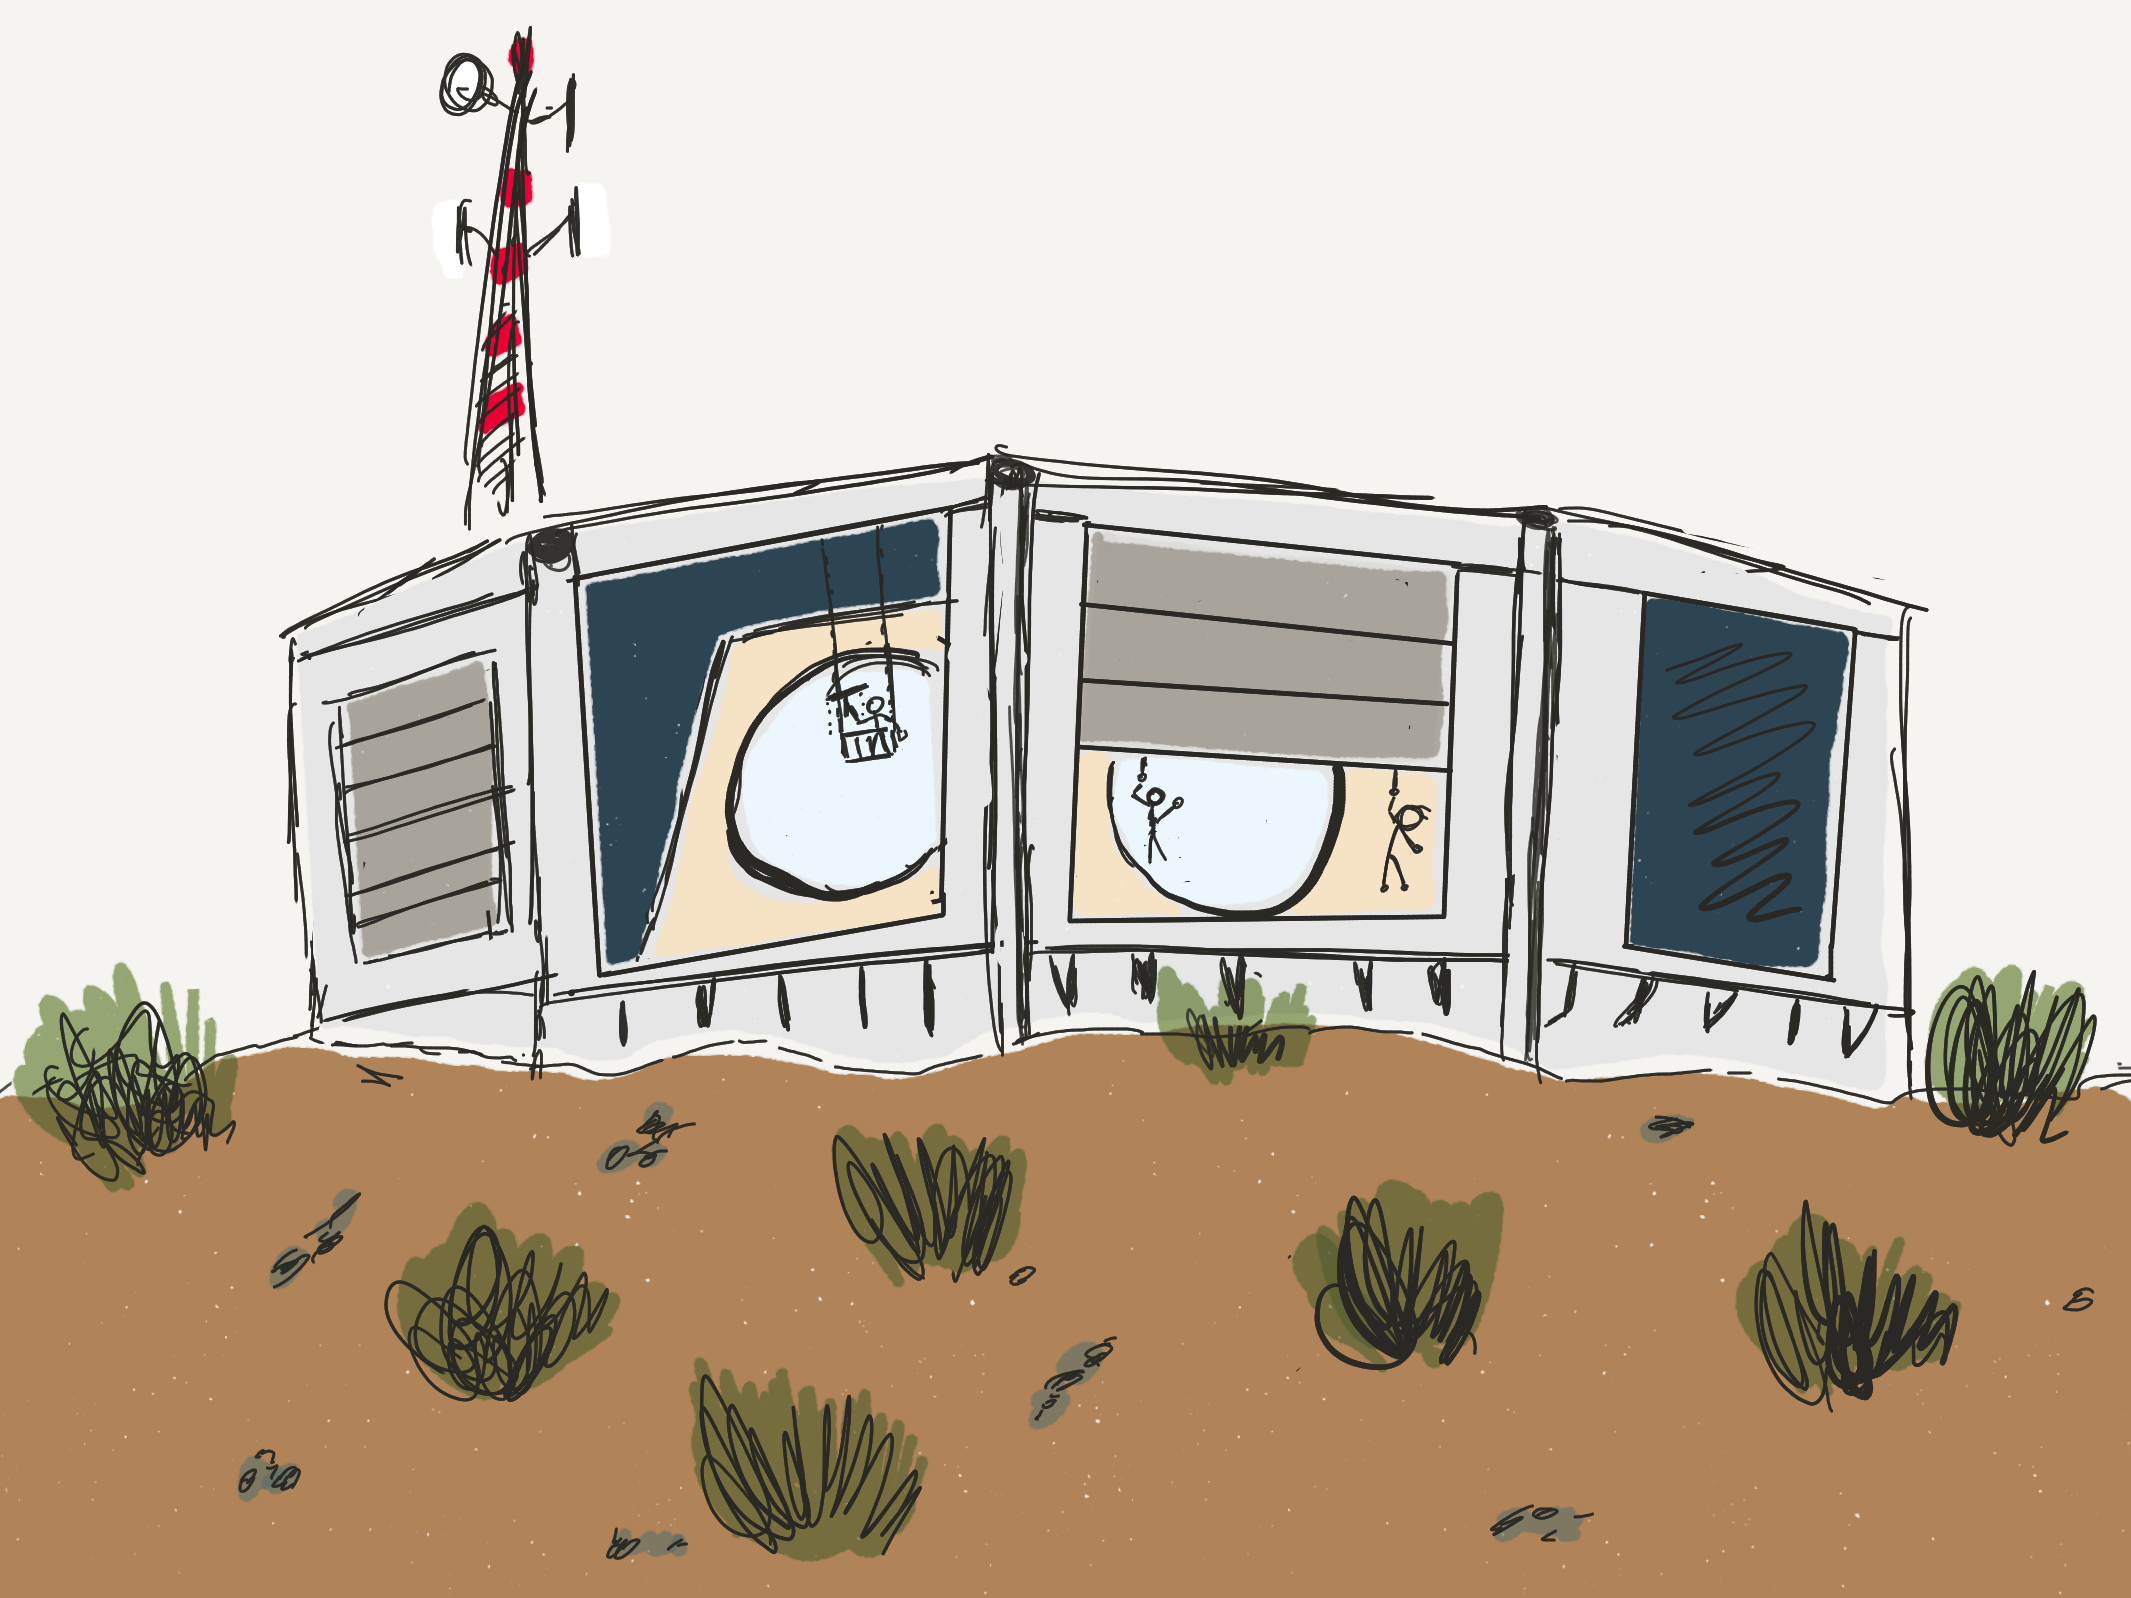
\includegraphics[width=.45\linewidth]{thesis_figures/Setup/FD_outside_drawing.png}}
  \hfill
  \subcaptionbox{Schematic view of a fluorescence telescope with a description of its main components taken from~\cite{Auger:2015}\label{sub:fig:FD_schematic}}{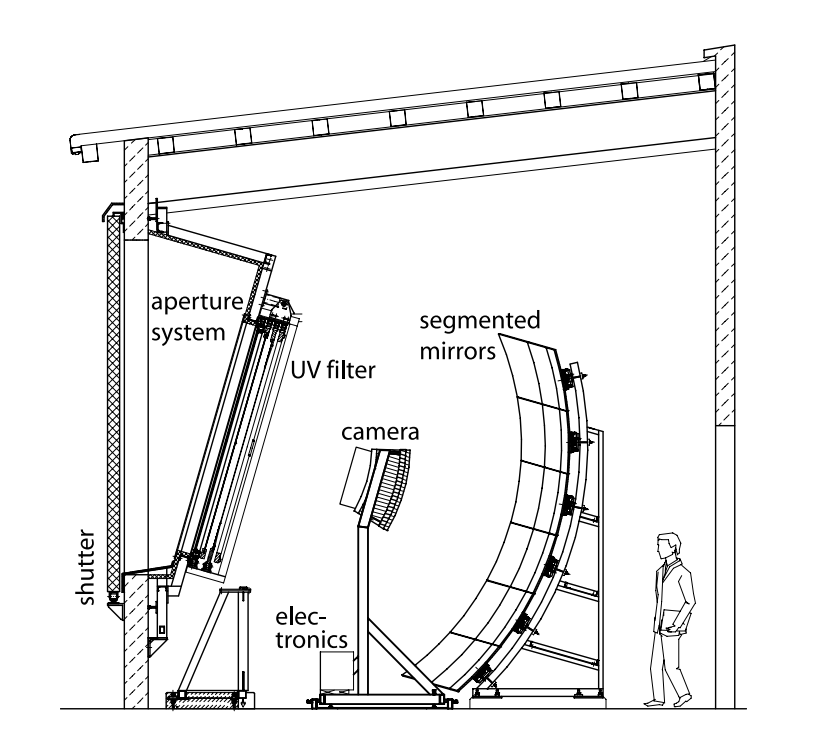
\includegraphics[width=.45\linewidth]{thesis_figures/Setup/FD_schematic.png}}
  \caption{Fluorescence Telescope at Pierre Auger Observatory}
  \label{fig:FD_sketch_schematic}
\end{figure}

Fig~\ref{fig:FD_sketch_schematic} shows an FD site along with the schematic of an FD telescope. The fluorescence light enters through the UV filtered window 
which is surrounded by a corrector ring. A spherical segmented mirror is used to gather the incoming light and focus it onto a 440 pixeled PMT camera. The camera records the light pulses every 100ns and based on a hierarchical trigger~\cite{Abraham_2010_FD} saves the event. For reconstructing the energy and the geometry of the shower the recorded information is combined with the information detected by the SD (hybrid) or other FD telescopes (stereo)~\cite{SALAMIDA2008207}. A relative calibration of the PMTs is performed for each camera before and after each night of data taking~\cite{Abraham_2010_FD}. A regular absolute calibration procedure called the X-Y scanner has also been developed and is currently being deployed at each FD telescope. 

The FD acts as an important calibration tool for the SD, especially for the energy estimation where the hybrid detection of EAS is used to provide a simulation free primary energy estimate for the SD. It can also be useful for looking into high energy atmospheric phenomena such as ELVES ~\cite{PierreAuger:2020lri}. The low duty cycle of the FD which is due to its operation being limited to clear moonless nights, limits its overall capabilities, especially for a neutrino analysis. However, the FD has been used for up-going neutrino searches (publication under review) and also has a potential use to look for atmosphere skimming CRs or neutrinos.  

\section{Surface Detector}
\label{sec:Sur_det}

\begin{figure}[h!]
  \centering
  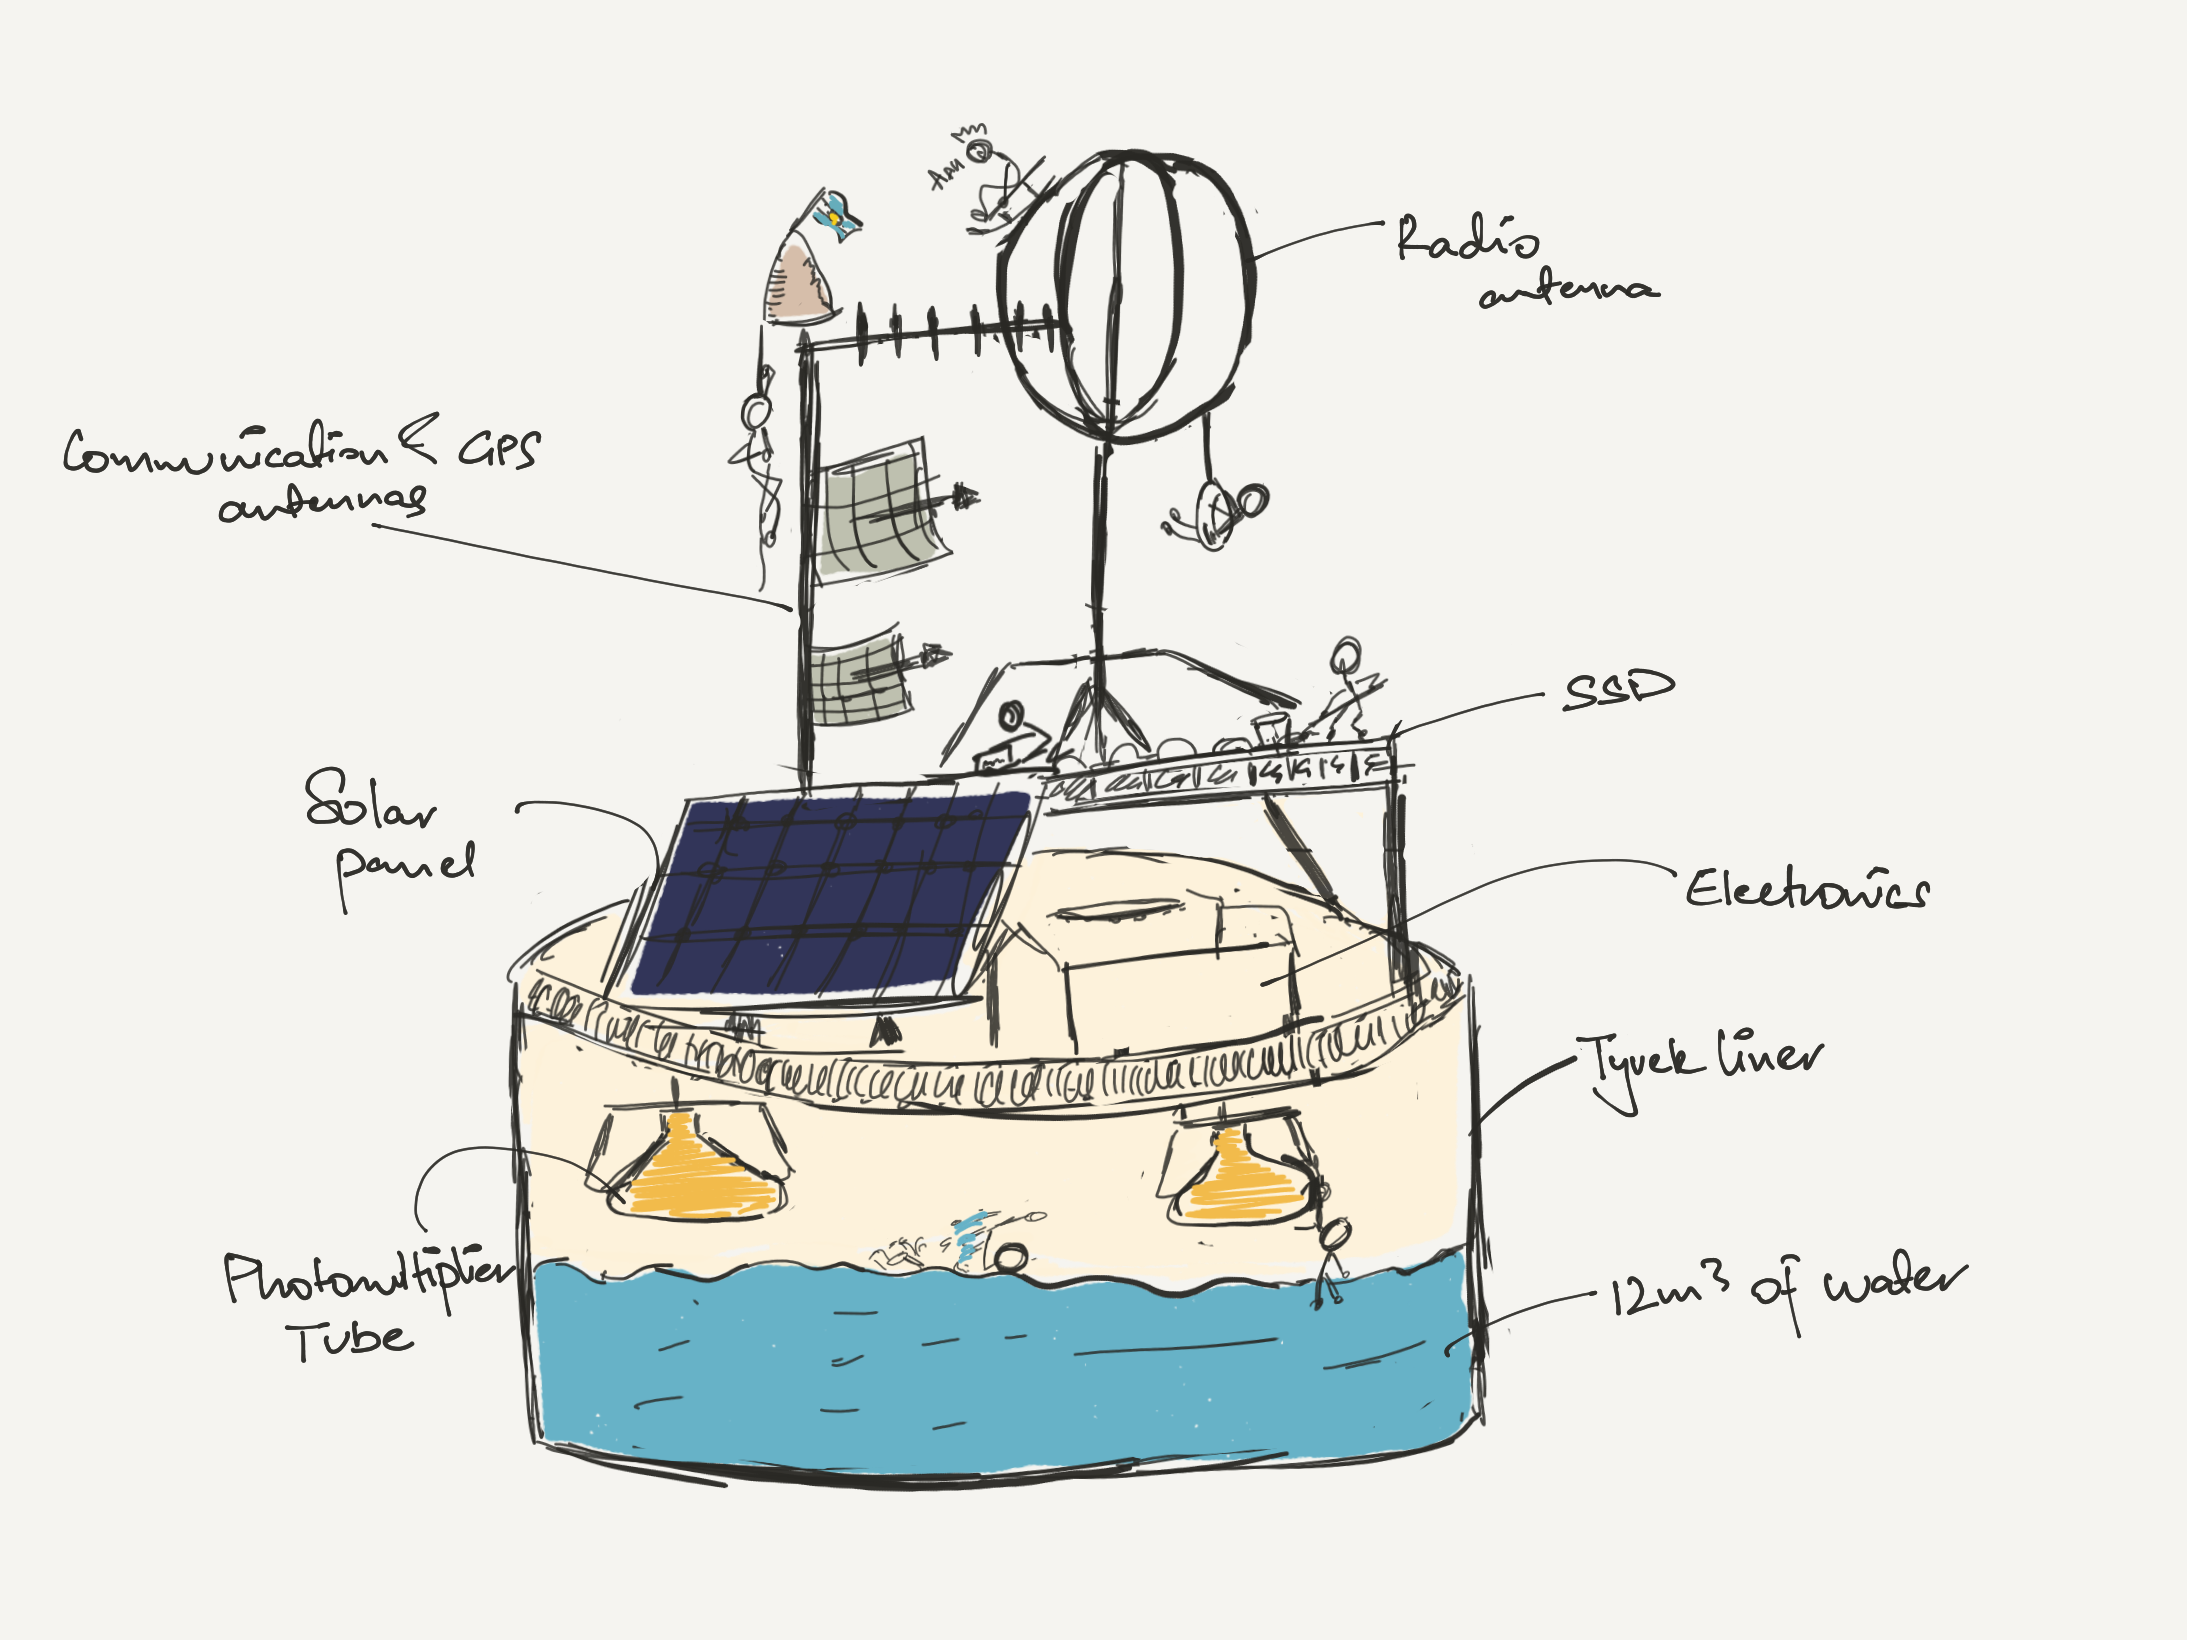
\includegraphics[width=\textwidth]{thesis_figures/Setup/SD_tank_schematics_drawing.png}
  \caption{Artistic representation of a Surface Detector tank with all its components with the AugerPrime upgrade. The third PMT and the small PMT are not visible in the drawing. The water level is usually touching the PMTs.}
  \label{fig:SD_drawing}
  \end{figure}

The \gls*{SD} baseline design consisted of a \gls{WCD} array which is used to detect the EAS on the ground by detecting the shower particles that reach the ground. Each WCD comprises of a tank with 3.6 m diameter and 1.2 m height~\cite{PierreAuger:2007kus}. It also consists of a reflective inner liner containing 12,000 litres of ultrapure water. Three 9-in PMTs look into the water and detect the Cherenkov light produced by the charged shower particles as they traverse through the water. With the AugerPrime upgrade the WCDs have also been equipped with a scintillator, additional PMT and a radio antenna on top. These are described later in section~\ref{sec:Aug_prime}. Each WCD tank also has its own electronics and communication system. All the components are powered using a solar panel. An artistic representation along with all the components is shown in Fig.~\ref{fig:SD_drawing}. 

The 1.5 km grid spacing is commonly referred to as SD-1500. There are further sub-arrays within the SD, SD-750 also called the infill and SD-433 with the numbers representing the distance between the tanks in the sub-arrays in meters. Each WCD can be operated on its own with each PMT signal first recorded at the station and then combined using a Central Data Acquisition System (CDAS)~\cite{Auger:2015} which uses a ranked system of triggers to decide if the combination of all WCDs is a candidate for an EAS event. The data taking process of the SD is described in more detail in the following sections. Due to its autonomous nature, the SD array is easy to maintain and has a duty cycle $\simeq$100\%. The array is only affected if there is a communication outage or if the solar panel cannot generate power for an extended time period both of which are rare at the site of the Pierre Auger Observatory. For this study whenever the SD is mentioned it refers to the SD-1500 array with only the WCD component unless specified otherwise.     

\subsection{Calibration of SD}
\label{sec:Sur_det_calib}

The PMT signals in the WCDs are digitised by a 40 MHz 10 bit \textit{\acrlongpl{FADC}} (\acrshortpl{FADC})~\cite{PierreAuger:2005znw}. One of the signals is taken from the anode of the PMT and is called the \textit{low gain} channel and the other is taken by the last dynode and is amplified by a factor of 32 and is called the \textit{high gain} channel. The two signals provide sufficient precision and range to record both the signals produced near the shower core ($\sim$1000 particles/$\mathrm{\mu}$s) and those produced far from the core ($\sim$1 particles/$\mathrm{\mu}$s). The signal trace is recorded at a sampling rate of 40 MHz with a total of 768 bins leading to each bin width corresponding to 25 ns. Due to varying electronics across the WCDs a robust procedure is needed to calibrate each station to a universal unit of measurement for the SD. Also, due to the remoteness of the WCDs such a procedure needs to be performed locally for each station to allow for its functioning even in the case of individual broken PMTs. The unit of measurement used to calibrate the SD stations is called \textit{\acrlong{VEM}} (\acrshort{VEM}). This is the charge deposited by a \gls{VCT} muon in the WCD station. The SD station by itself cannot select these particular muons but the normal SD measurement of all atmospheric muons has been studied in comparison with a muon telescope that only triggers these VCTs for a reference tank~\cite{PierreAuger:2005cju}. This measurement is used to calibrate the SD.

\begin{figure}[h!]
  \centering
  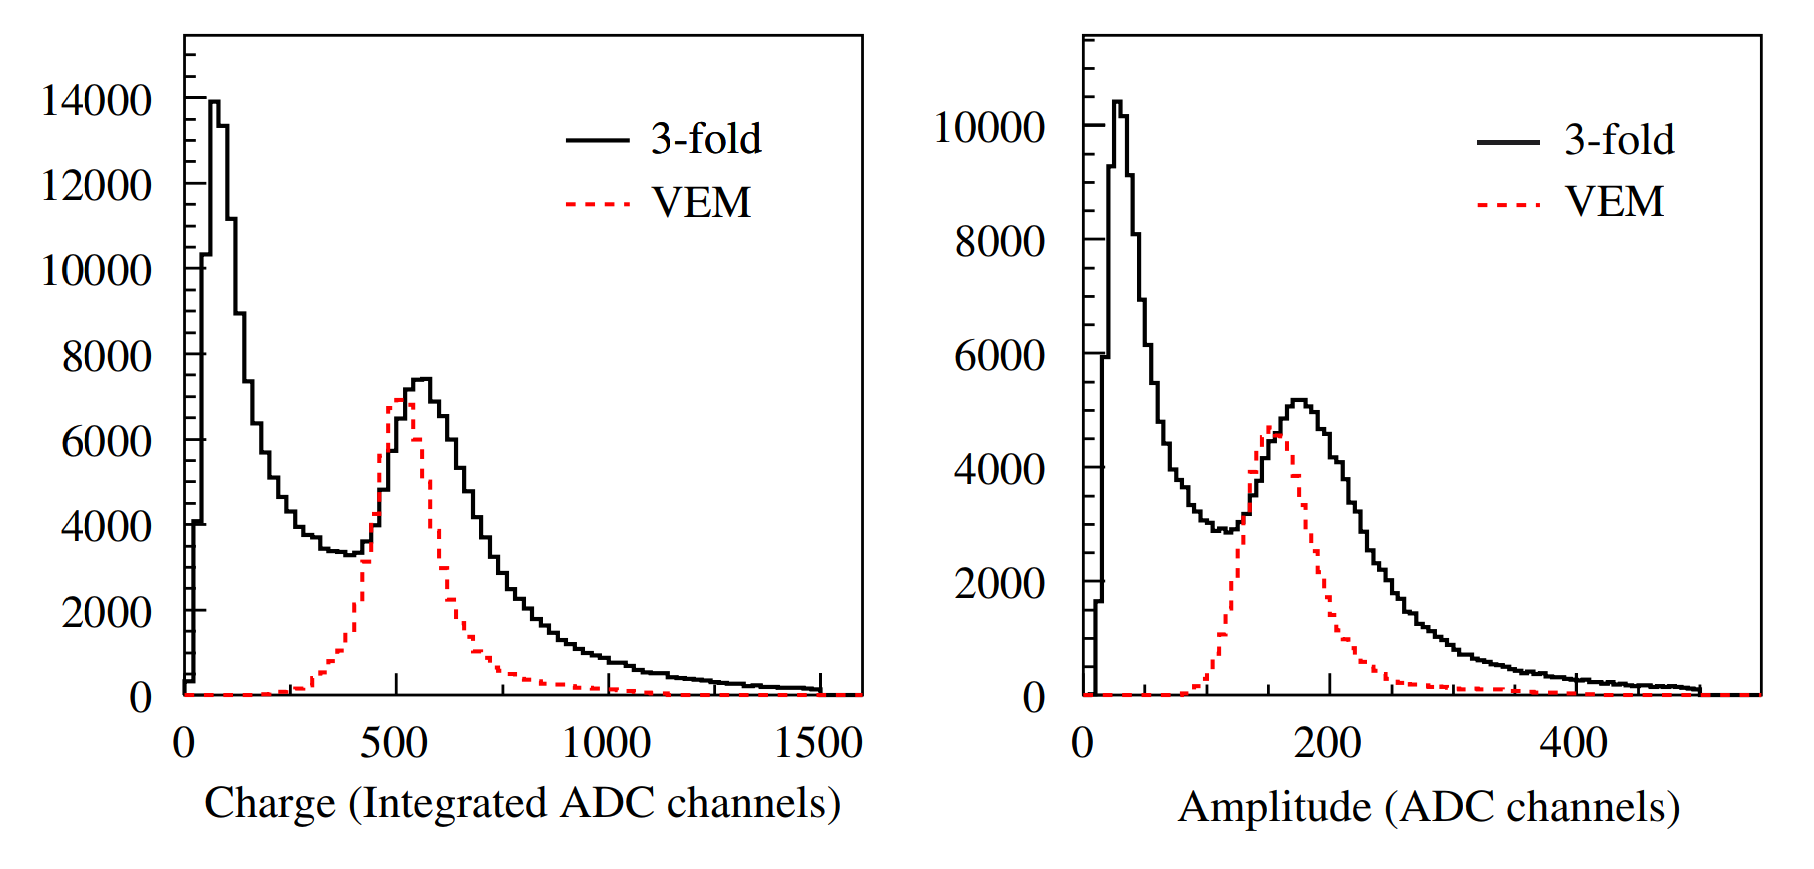
\includegraphics[width=\textwidth]{thesis_figures/Setup/VEM_Calib_SD.png}
  \caption{Left:The charge histogram (black), is the sum of the responses of all three
  PMTs above the electronic noise threshold, while the dashed red line
  represents the reference measurement done by an external muon telescope.
  The first peak in the charge histogram is noise from low-energy particles. The second peak is caused by the vertical-through going muons and is used to determine VEM. Right: The pulse height histogram (black) that is
  used to calibrate $I^{\text{peak}}_{\text{VEM}}$ which is used for trigger thresholds. The calibration is again performed using the reference measurements from the muon telescope.~\cite{PierreAuger:2005znw}}
  \label{fig:SD_VEM_calib}
\end{figure}

To perform the calibration charge distribution, $Q_{\text{VEM}}^{\text{peak}}$, and the pulse height, $I_{\text{VEM}}^{\text{peak}}$, both for the individual PMTs and their sums, are compared to the measurements done with a muon telescope as shown in Fig.~\ref{fig:SD_VEM_calib}. The first peak in the figure for the PMT measurement is caused due to low energy particles while the second peak is produced by the atmospheric muons. This peak corresponds to $Q_{\text{VEM}}^{\text{peak}}$ $\simeq$ 1.03 VEM for the sum and $\simeq$1.09 VEM for each PMT. The shift in comparison to the muon telescope measurement is caused by the convolution of photo-electron statistics on an asymmetric peak in the track length distribution and local light collection effects. This peak is used to obtain a conversion for the integrated signal of the PMT to VEM units. In addition to this, since the subsequent trigger for the SD also requires a measure of the current $I_{\text{VEM}}$, this value also needs to be converted and calibrated to VEM units~\cite{PierreAuger:2005znw}. The same technique as the charge calibration is employed since the VCTs also produce a peak in the pulse height histograms. The calibration is performed every 60 s and sent to CDAS thus for an incoming event, calibration data is available for the preceding minute ensuring high calibration accuracy. 

\subsection{SD Trigger system}
\label{sec:Sur_det_trig}
A schematic of the logic of the trigger system is shown in fig~\ref{fig:SD_trigger_logic}. There are three types of different types of station level triggers scalar, calibration and shower trigger. The scalar trigger records signals for very low thresholds and is useful for supplementary physics such as space weather~\cite{Dasso:2012vk}. The calibration trigger, as explained in the previous section, helps store and calculate the calibration parameters. The main shower trigger, used to record the EAS events is a hierarchical system consisting of two local triggers (T1 and T2) implemented at the station level, a third level trigger (T3) implemented by CDAS and further event selection triggers (T4 and T5) stored by the SD but only used depending on the analysis and the quality of data required by the said analysis. The hierarchical nature arises from the limits on the wireless communication network required for a vast autonomous array. The T3 trigger aims to reduce the rate especially for the expected muonic background and at the same time maximising the EAS event detection.  

\begin{figure}[h!]
  \centering
  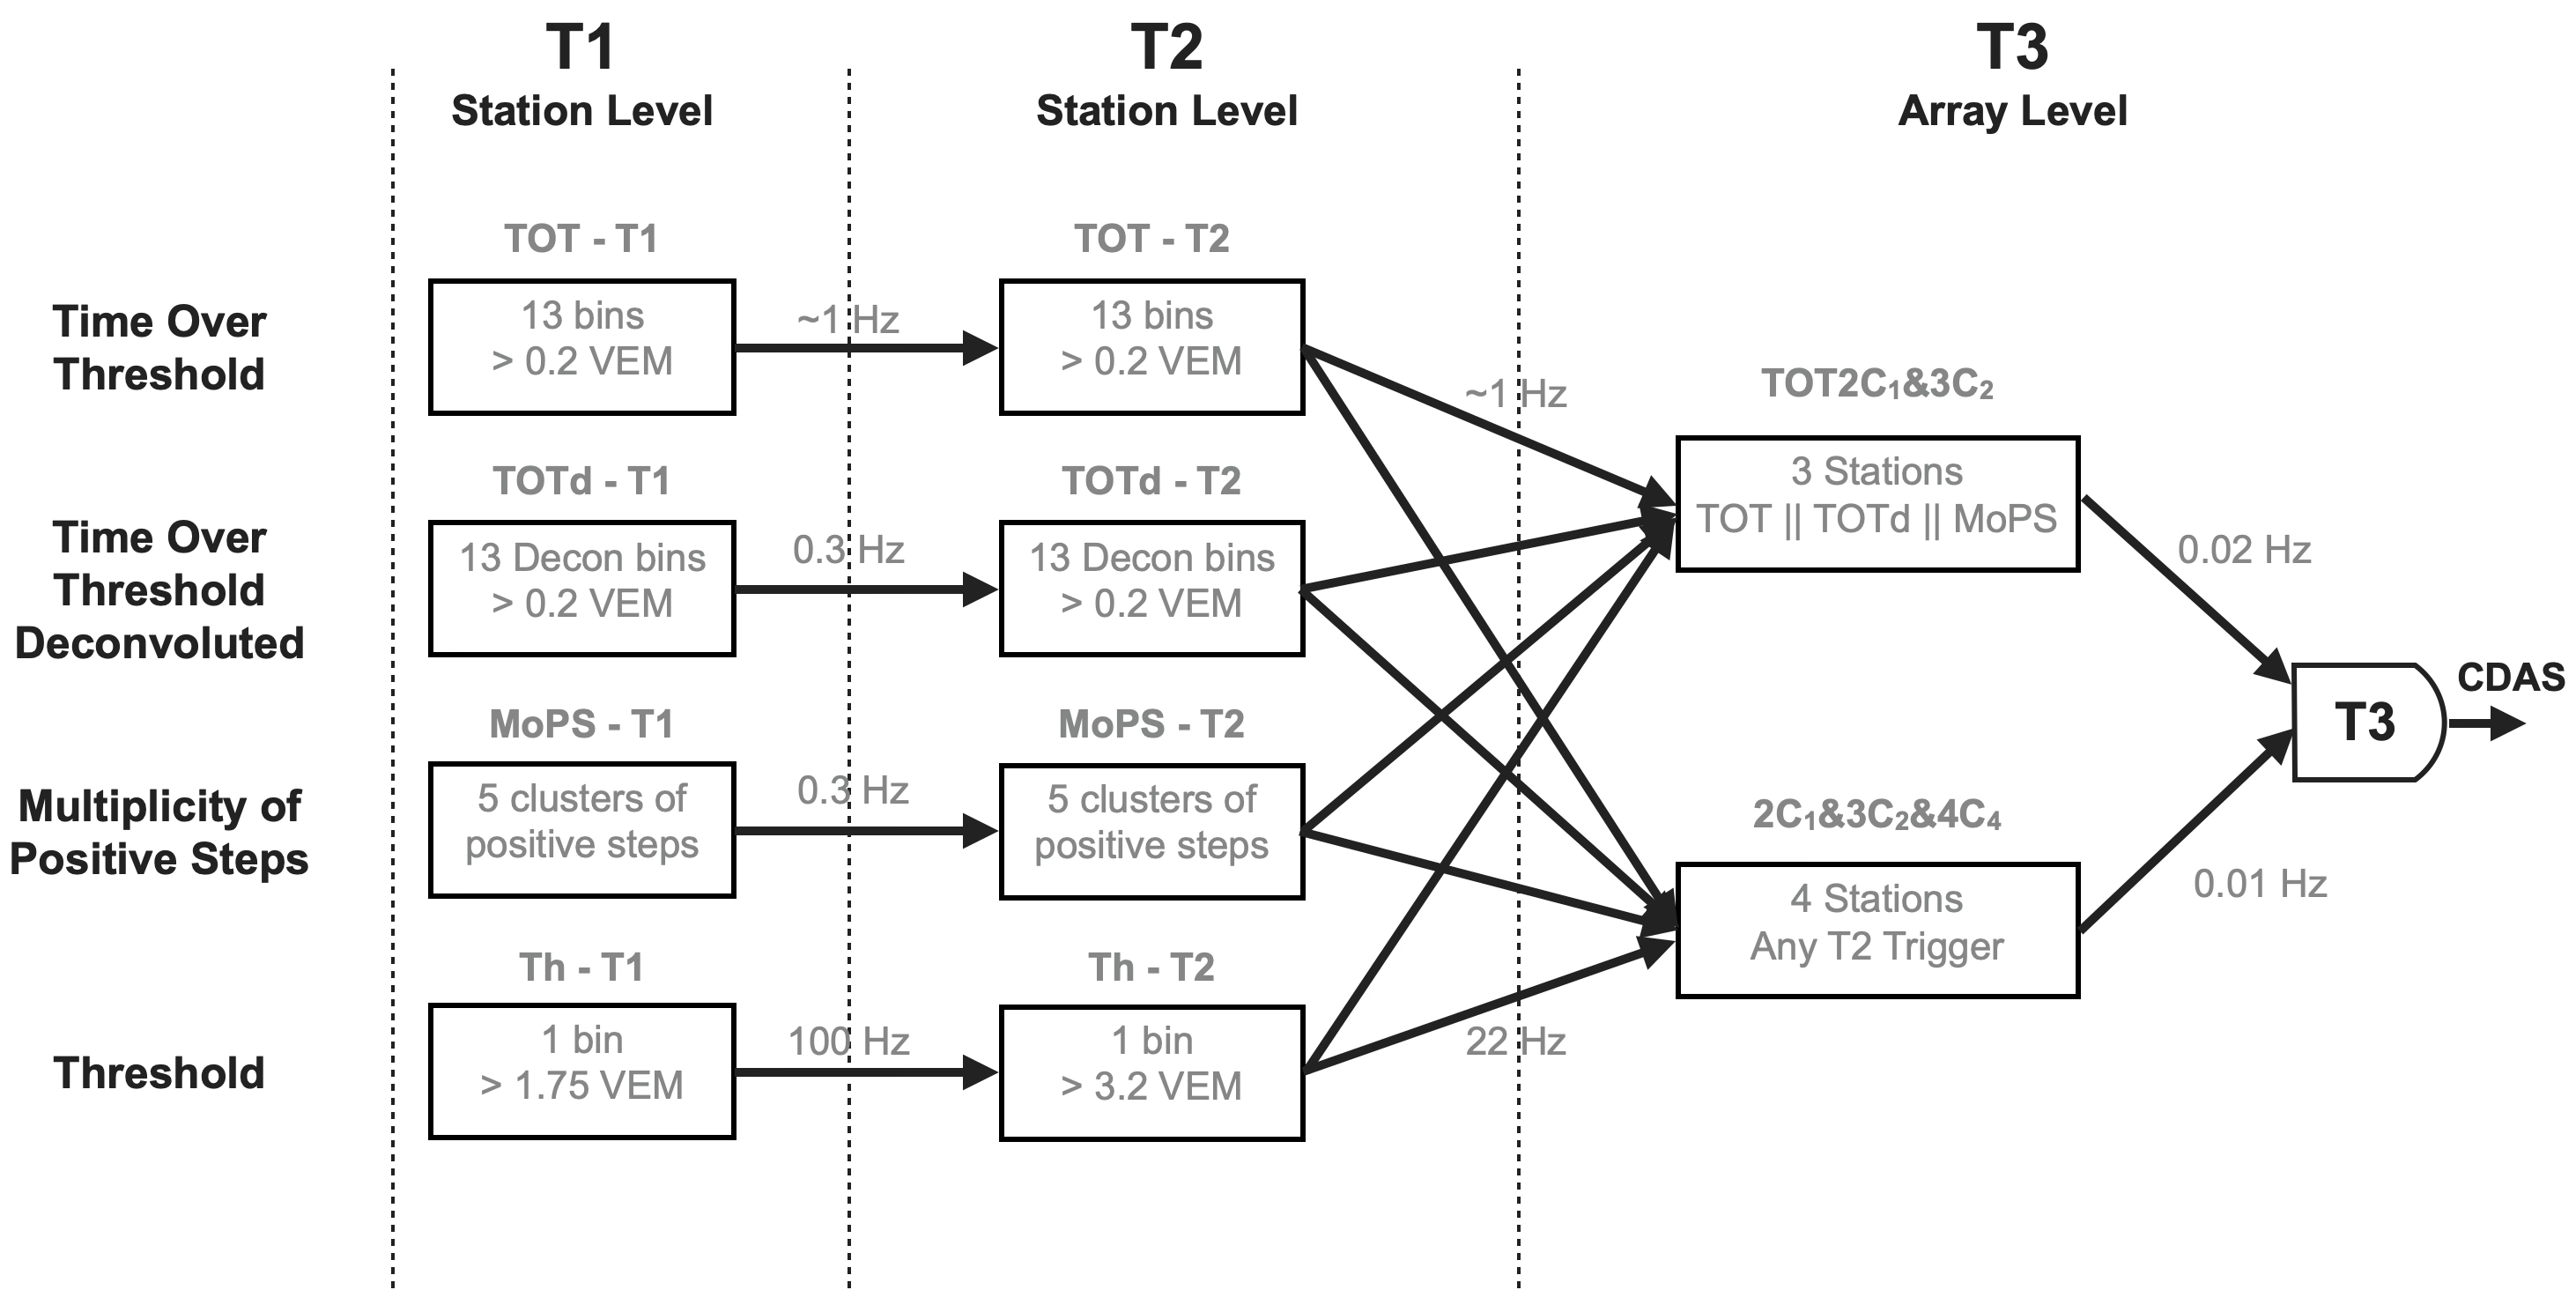
\includegraphics[width=\textwidth]{thesis_figures/Setup/Trigger_logic.png}
  \caption{Schematics of the hierarchy of the trigger system of the Auger surface detector.}
  \label{fig:SD_trigger_logic}
\end{figure}

\subsubsection{Old triggers}
\label{sec:Sur_det_trig_old}
The T1 trigger consists of two parts/modes both of which need to be satisfied for an event to be checked for the possibility of higher level triggers. One of them is a basic \gls{TH} that requires the signal for each of the three PMTs to be above 1.75$I_{\text{VEM}}^{\text{peak}}$. If there are only one or two PMTs active then the requirement changes to >2.8$I_{\text{VEM}}^{\text{peak}}$ or >2$I_{\text{VEM}}^{\text{peak}}$ respectively. The TH mode is used to select large signals which are expected for very inclined CR induced showers ($\theta >60^{\circ}$) which are predominantly muons. It reduces the rate for the atmospheric muons from 3 KHz to a 100 Hz. The second mode for the T1 trigger is called \gls{ToT}. ToT requires 13 or more of the 25 ns time bins within a 3$\mu$s window to be above a threshold of 0.2$I_{\text{VEM}}^{\text{peak}}$ for at least two PMTs. Since this mode filters for signals spread in time it is sensitive to low energy vertical showers nearer to the core and also high energy inclined showers far from the shower core. It is also very effective in filtering random muonic background which typically has a spread of 150ns compared to the 325 ns spread for ToT fulfilment. The rate for ToT at each detector is $\sim$1.2 KHz with the main contribution being two consecutive muons arriving within the time window. 

\subsubsection{New triggers}
\label{sec:Sur_det_trig_new}
In June 2013, two additional T1 trigger modes were implemented at the Pierre Auger Observatory to reduce the influence of atmospheric background muons and reduce the energy threshold of the array. The two modes both of which build upon the ToT condition are time-over-threshold-deconvolved (ToTd) and multiplicity-of-positive-steps (MoPS).

The ToTd trigger was first proposed internally in~\cite{gap_note_2009}. The trigger aims to deconvolve the FADC trace, suppressing the exponential tail of the diffusely reflected Cherenkov emission before applying the ToT condition. This helps in compressing the signal from a muon which typically has a fast rise time in one or two time bins before the application of the ToT condition. The trigger has an expected rate of 0.2 Hz-3 Hz. ToTd also requires the integrated signal to be above 0.5 VEM. An example of the functioning of the trigger is shown in Fig.~\ref{fig:ToTd+MoPSworking}. 

% \begin{figure}[t!]
%   \centering
%   \begin{subfigure}[b]{0.45\textwidth}
%       \centering
%       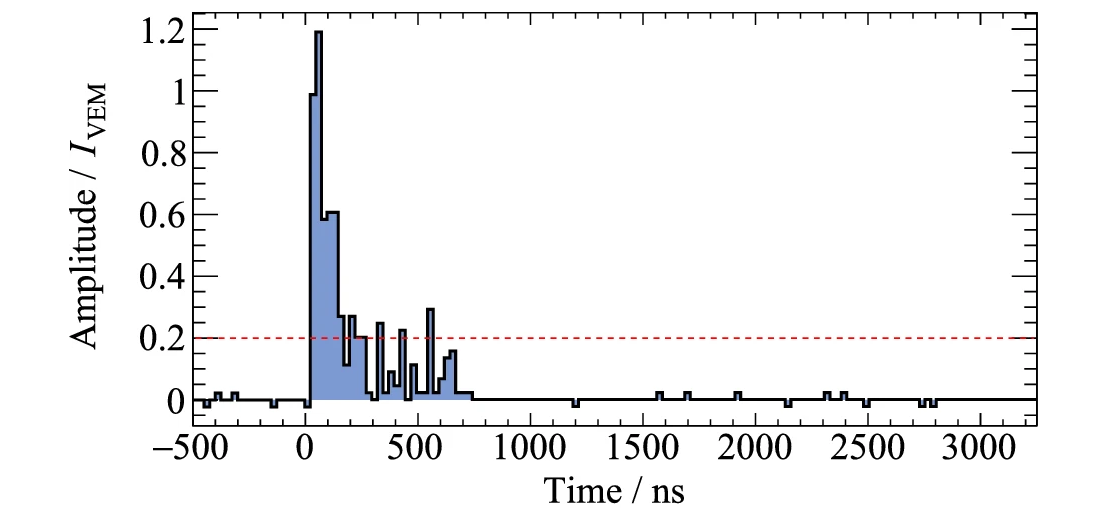
\includegraphics[width=\textwidth]{thesis_figures/Setup/Totd.png}
%       \caption{Example waveform which passes the ToTd algorithm.}
%       \label{sub:fig:FD_site_drawing}
%   \end{subfigure}
%   \hfill
%   \begin{subfigure}[b]{0.45\textwidth}
%       \centering
%       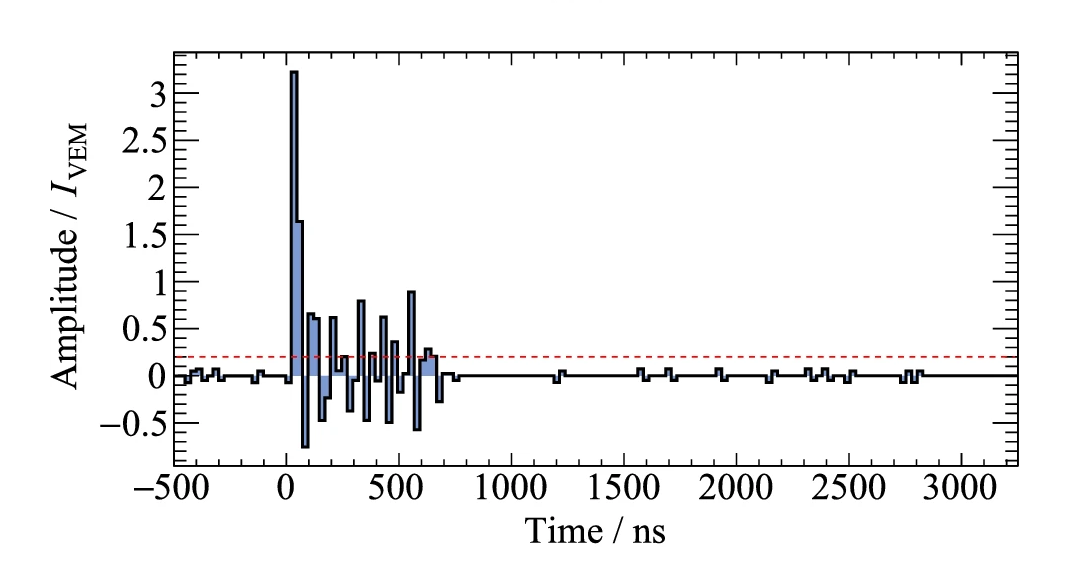
\includegraphics[width=\textwidth]{thesis_figures/Setup/Ttd_deconvuluted.png}
%       \caption{The deconvolution of the initial ToTd waveform along with the required threshold in red dashed line}
%       \label{sub:fig:FD_schematic}
%   \end{subfigure}
%      \caption{Functioning of ToTd trigger. Taken from~\cite{PierreAuger:2021hun}}
%      \label{fig:ToTd_working}
% \end{figure}

\begin{figure}
  \centering
  \subcaptionbox{Example waveform which passes the ToTd algorithm.\label{sub:fig:ToTd_example}}{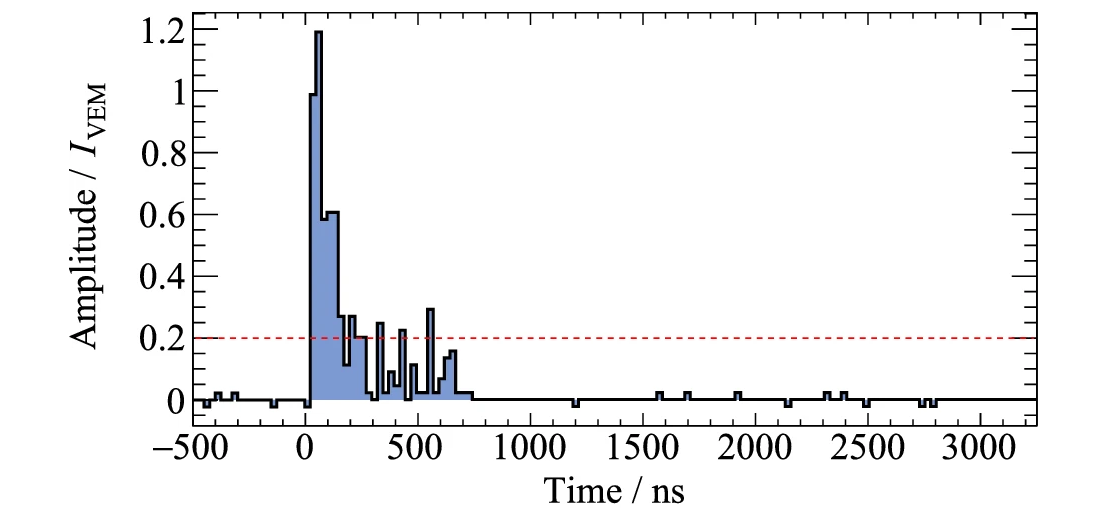
\includegraphics[width=.45\textwidth]{thesis_figures/Setup/Totd.png}}
  \hfill
  \subcaptionbox{The deconvolution of the initial ToTd waveform along with the required threshold in red dashed line\label{sub:fig:ToTd_working}}{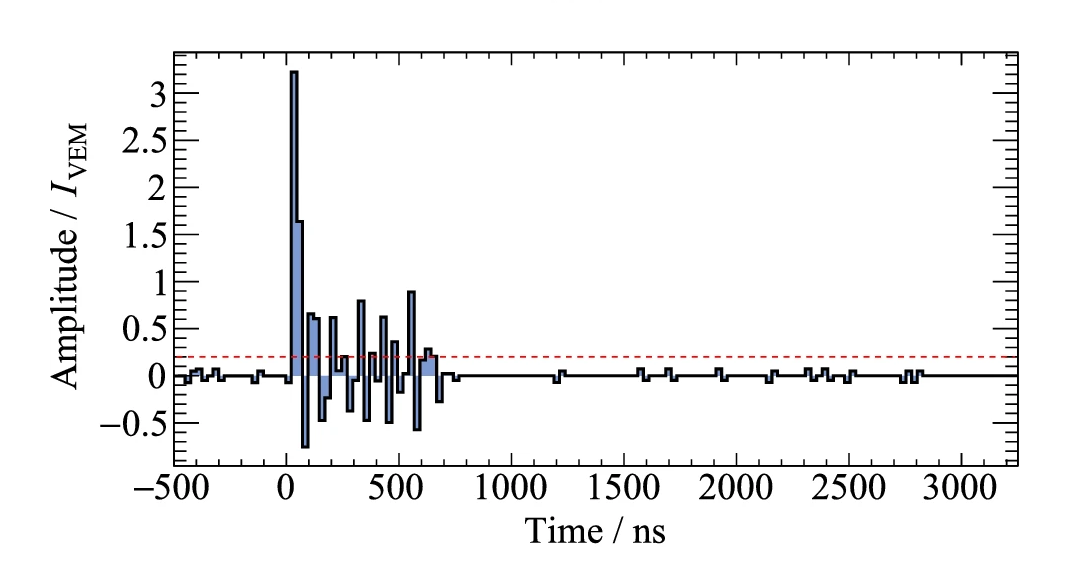
\includegraphics[width=.45\textwidth]{thesis_figures/Setup/Ttd_deconvuluted.png}}
  \subcaptionbox{Example waveform which passes the MoPS algorithm.\label{sub:fig:MoPS_working}}{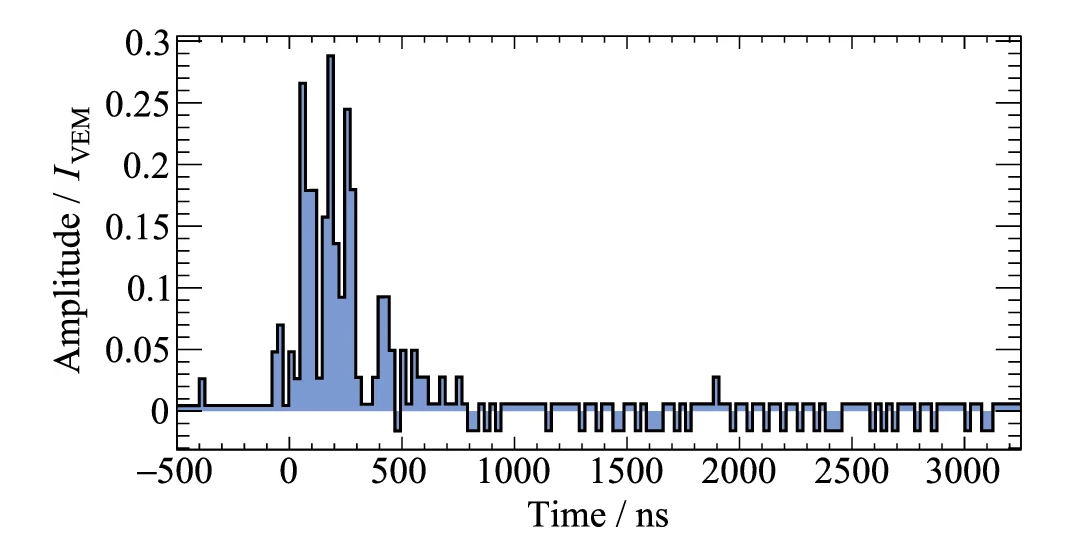
\includegraphics[width=.45\textwidth]{thesis_figures/Setup/MoPS.png}}
  \caption{Functioning of ToTd trigger and an example of MoPS. Taken from~\cite{PierreAuger:2021hun}}
  \label{fig:ToTd+MoPSworking}
\end{figure}

The MoPS trigger~\cite{gap_note_2011} was implemented to achieve a similar goal as ToT and ToTd i.e. a better separation between the air shower signal from the mostly muonic background. It is designed to do so by counting the number of positive steps (cumulation of successive increases) in the \gls{FADC} trace within a 3 $\mu$s sliding window. These steps are expected to be above a certain threshold (5xRMS noise) and below a maximum value ($\sim$0.5 VEM). The MoPS trigger is satisfied if more than 4 positive steps are counted during the sliding window in at least 2 PMTs. The expected rates both from simulations and data taking are found to be <2 Hz. MoPS is even better at recovering lower signals compared to ToT and ToTd, thus improving the overall trigger efficiency. Both ToTd and MoPS are implemented as an OR logic with the ToT condition. An example of a signal that passes the MoPS trigger is shown in Fig.~\ref{sub:fig:MoPS_working}.

% \begin{figure}[t!]
%   \centering
%   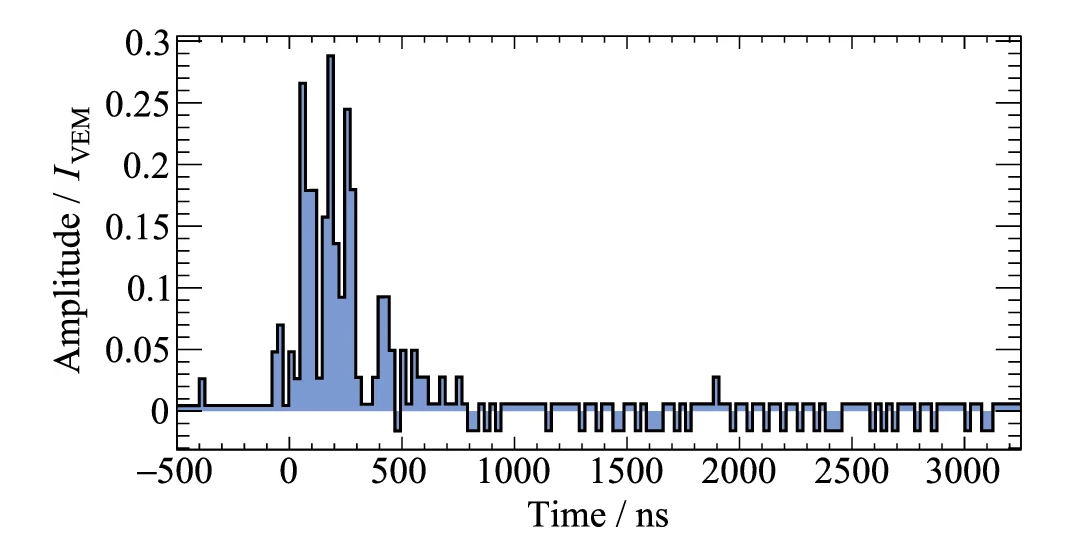
\includegraphics[width=0.75\textwidth]{thesis_figures/Setup/MoPS.png}
%   \caption{Example waveform which passes the MoPS algorithm.}
%   \label{fig:MoPS_working}
% \end{figure}

% \begin{figure}[t!]
%   \centering
%   \begin{subfigure}[b]{0.45\textwidth}
%       \centering
%       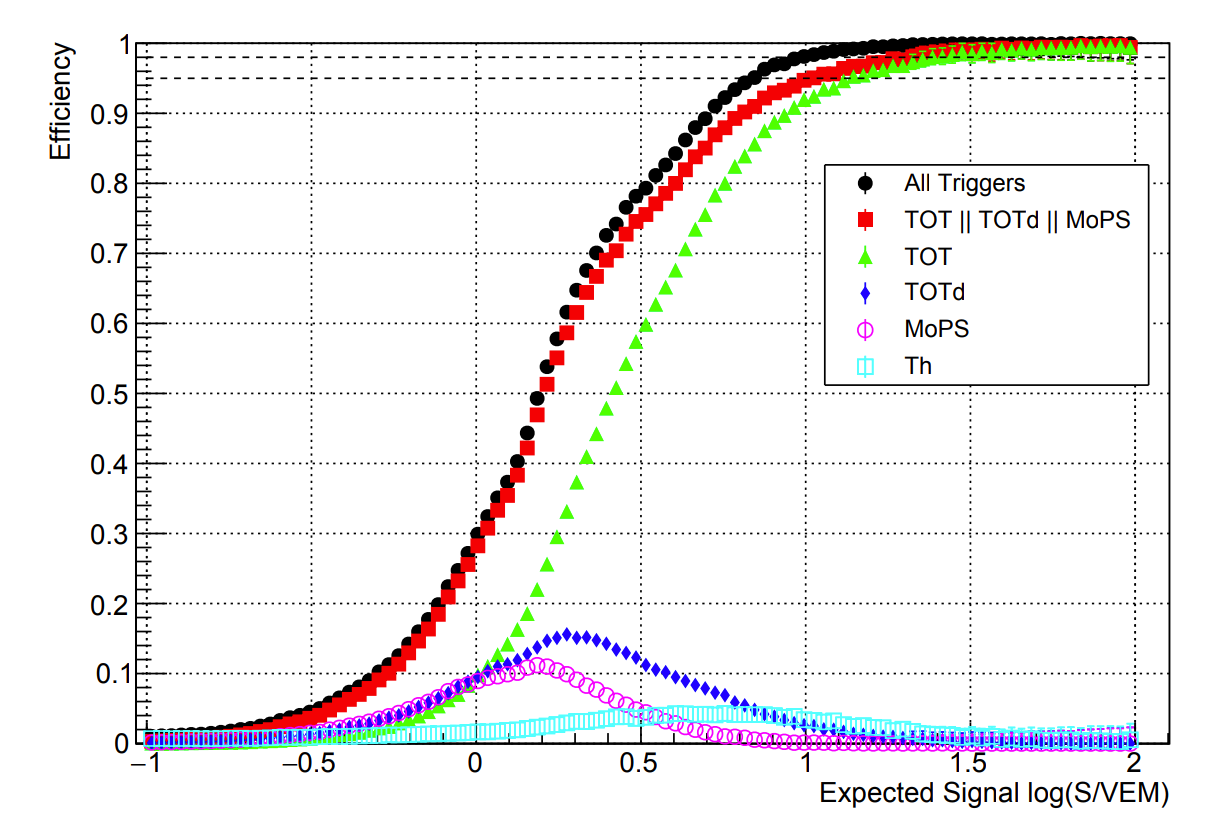
\includegraphics[width=\textwidth]{thesis_figures/Setup/Efficiency_triggers.png}
%       \caption{ Contribution to the different triggers to the efficiency as a function
%       of the mean expected signal. Respectively green, blue, pink and cyan
%       for TOT, TOTd, MOPs and Th.}
%       \label{sub:fig:Triiger_eff_infill}
%   \end{subfigure}
%   \hfill
%   \begin{subfigure}[b]{0.45\textwidth}
%       \centering
%       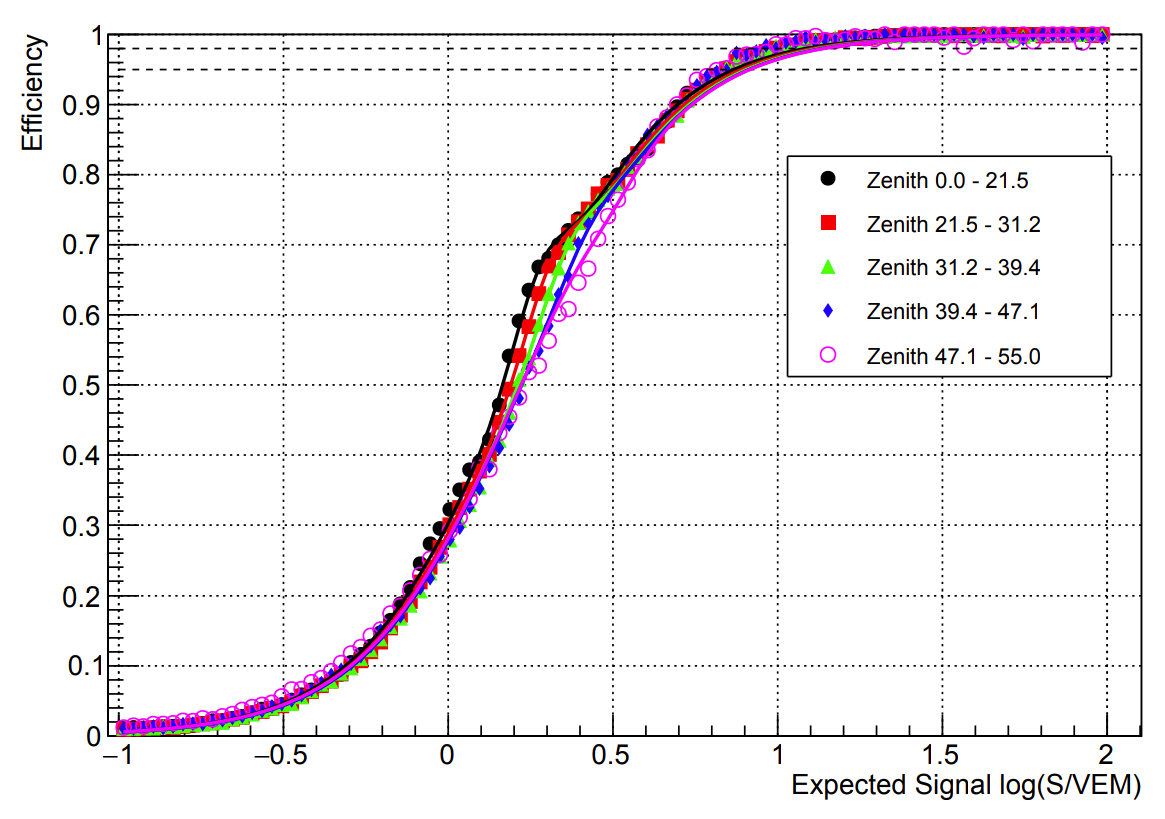
\includegraphics[width=\textwidth]{thesis_figures/Setup/Triggering_efficiency_theta.png}
%       \caption{The change in the triggering efficiency with zenith angle.}
%       \label{sub:fig:Trigger_eff_theta}
%   \end{subfigure}
%      \caption{Trigger efficiency for different triggers implemented at the Pierre Auger Observatory calculated using the SD-750 array for zenith angles below $60^{\circ}$. Taken from~\cite{PierreAuger:2021hun}}
%      \label{fig:Trigger_eff_infill}
% \end{figure}

\begin{figure}[t!]
  \centering
  \subcaptionbox{Contribution to the different triggers to the efficiency as a function
  of the mean expected signal. Respectively green, blue, pink and cyan
  for ToT, ToTd, MOPs and Th.\label{sub:fig:Triiger_eff_infill}}{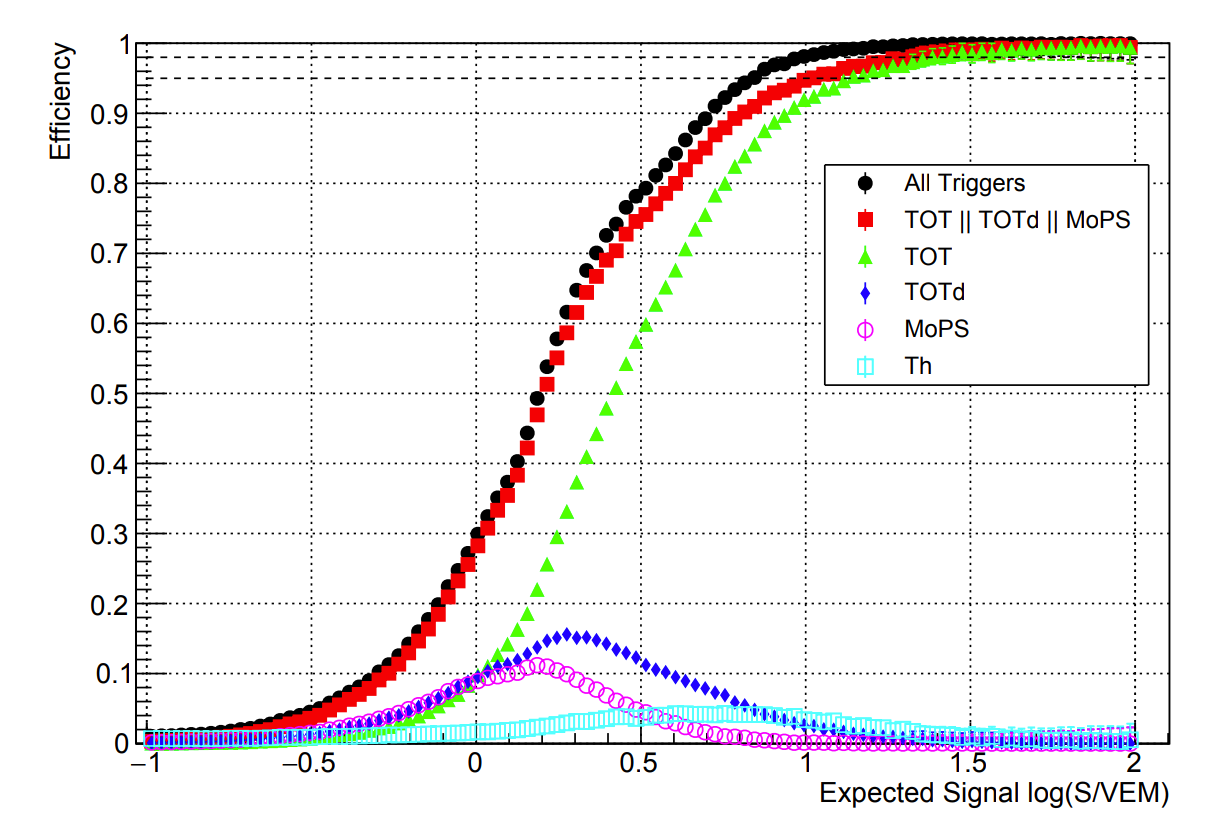
\includegraphics[width=.45\textwidth]{thesis_figures/Setup/Efficiency_triggers.png}}
  \hfill
  \subcaptionbox{The change in the triggering efficiency with zenith angle.\label{sub:fig:Trigger_eff_theta}}{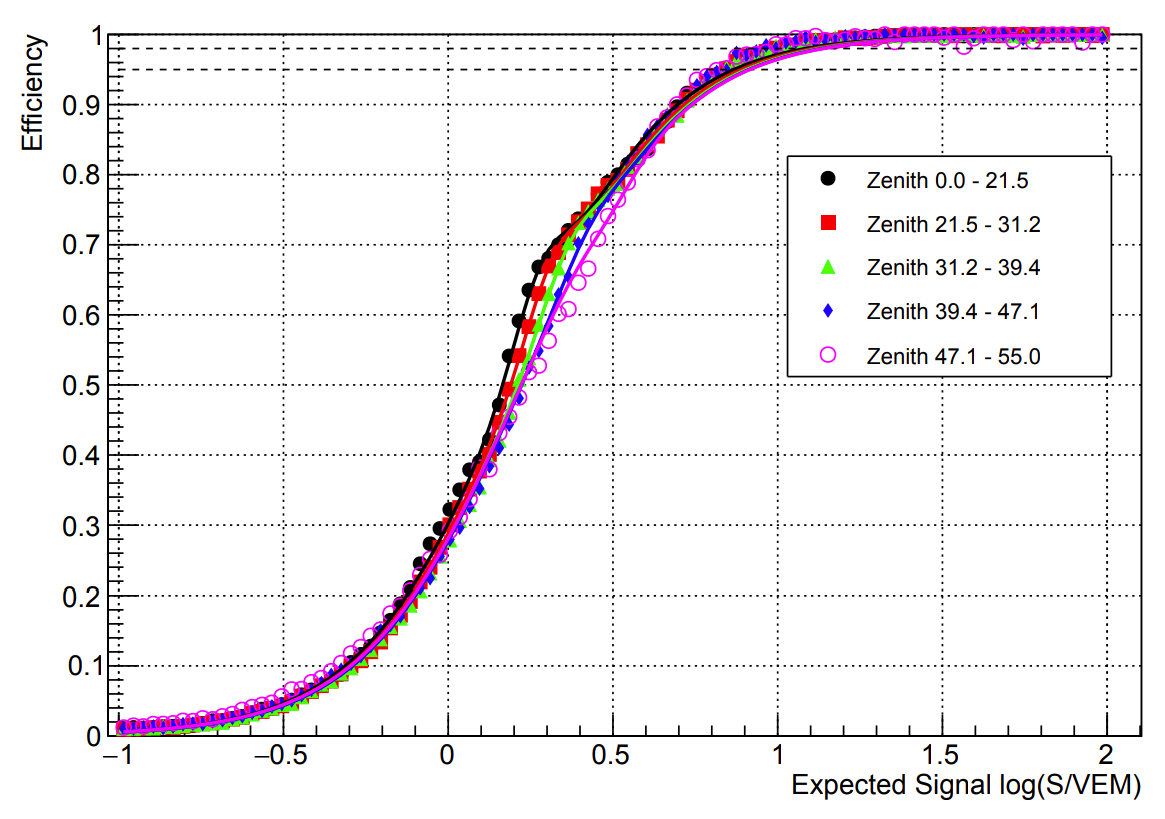
\includegraphics[width=.45\textwidth]{thesis_figures/Setup/Triggering_efficiency_theta.png}}
  \caption{Trigger efficiency for different triggers implemented at the Pierre Auger Observatory calculated using the SD-750 array for zenith angles below $60^{\circ}$. Taken from~\cite{gap_note_2017}}
  \label{fig:Trigger_eff_infill}
\end{figure}

The trigger efficiencies for the different T1s implemented at the Pierre Auger Observatory along with the zenith dependence are shown in Fig.~\ref{fig:Trigger_eff_infill}. The results are taken from a study~\cite{gap_note_2017} performed over three years using a special doublet hexagon which consisted of two hexagons of SD stations next to each other, one with new triggers active and one with new triggers inactive. Due to the small size of the hexagon the study was only performed for zenith angles less than $60^{\circ}$. However, the overall trend i.e. increase in efficiency holds for higher zenith angles. This is validated in sec.~\ref{sec:reco_possel} where an overall increase in events is seen when new triggers are included in the neutrino analysis.

The new triggers particularly improve the trigger efficiency and sensitivity for photon and neutrino induced EAS. By rejecting the signals caused by muons or other low energetic particles the new triggers are expected to increase the low energy threshold for the detection of these particles. They also help in recording more low electromagnetic like signals which is the expected signature for photons and neutrinos. 

\begin{figure}[t!]
  \centering
  \subcaptionbox{ToT2C$_1$\& 3C$_2$\label{sub:fig:T3_config_1}}{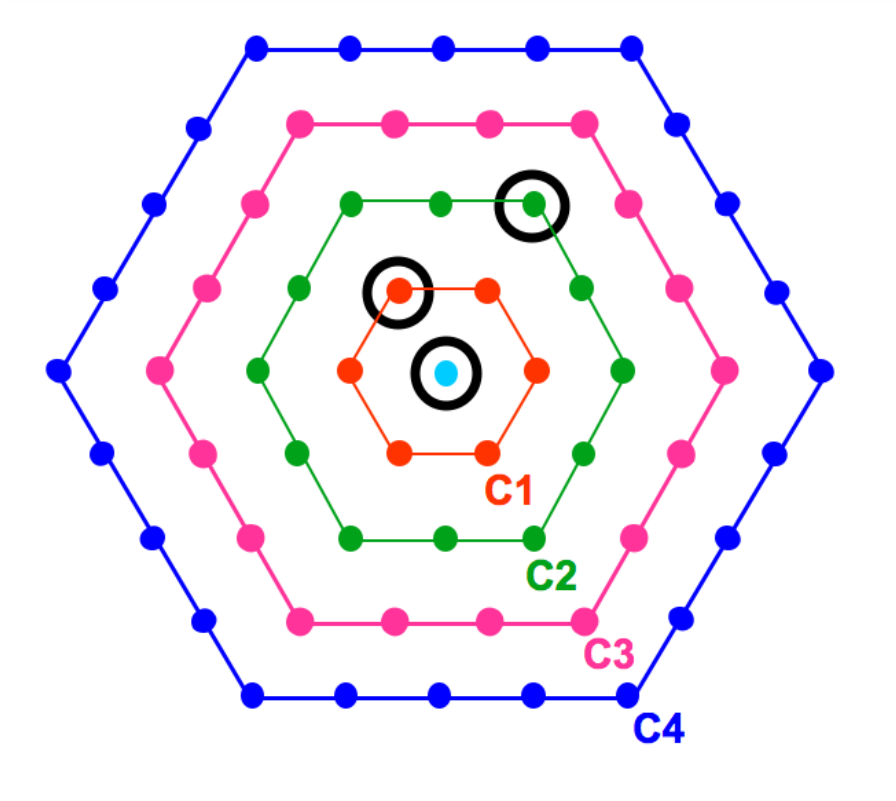
\includegraphics[width=.45\linewidth]{thesis_figures/Setup/T3_config_1.png}}
  \hfill
  \subcaptionbox{2C$_1$\&3C$_2$\&4C$_4$\label{sub:fig:T3_config_2}}{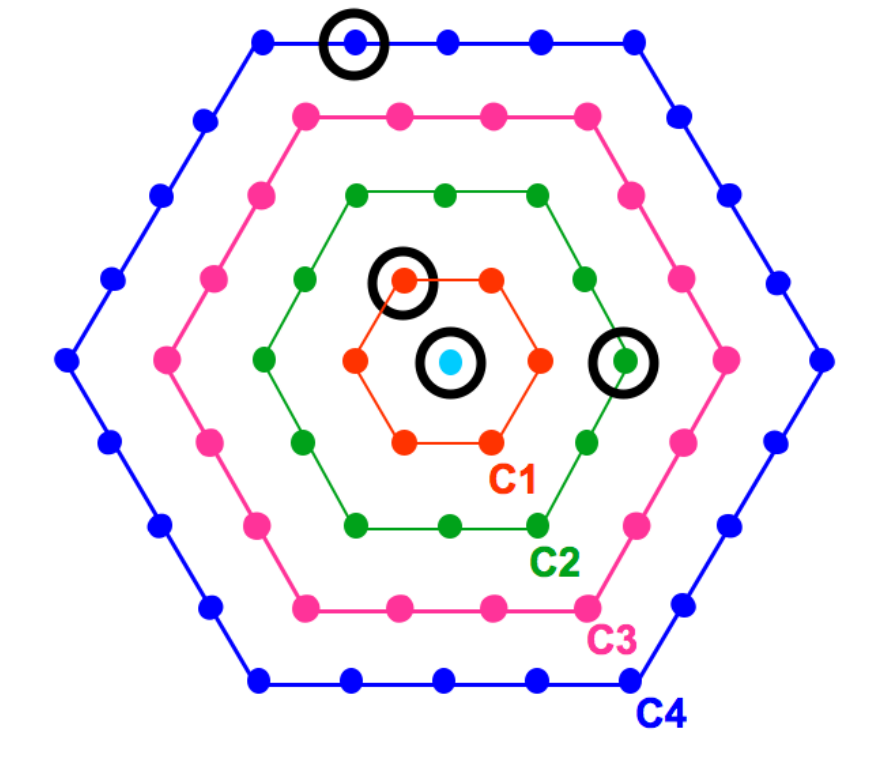
\includegraphics[width=.45\linewidth]{thesis_figures/Setup/T3_config_2.png}}
  \caption{Example of two possible T3 configurations. Taken from~\cite{PierreAuger:2010zof}}
  \label{fig:T3_config}
\end{figure}

\subsubsection{Array Level Triggers}
\label{sec:Sur_det_trig_array}
T2 level triggers aim to apply higher constraints to T1 triggers. A T1-ToT trigger is automatically updated to a T2-ToT trigger while a T1-TH trigger requires the signal to pass a higher threshold condition of >3.2$I_{\text{VEM}}^{\text{peak}}$ for three coincident PMTs to get upgraded to T2-TH. For two (one) working PMTs the threshold is stricter at >3.8 (4.5)$I_{\text{VEM}}^{\text{peak}}$. After the T2 level, the expected station rate of events drops to $\sim$23 Hz. The T2 level triggers from all stations are sent to the CDAS to form a global trigger.

The T3 level aims to build a condition based on both spatial and temporal combinations of stations that have passed the T2 condition. It again has two modes with only one needed to be satisfied to form a successful T3. Both of these conditions use a unit of detector called the crown, $C_n$. The crown as shown in Fig.~\ref{fig:T3_config} is a set of concentric hexagons centred around each station with $n$ giving the order of the surrounding hexagons, 1 being the nearest. The first mode $ToT2C_1\&3C_2$ (\ref{sub:fig:T3_config_1}) requires three SD stations which have passed T2-ToT criteria. It further requires at least one station to be located in the first crown denoted by $2C_1$ and the last to be located in the second crown ($3C_2$). The trigger is efficient in selecting compact vertical showers ($\theta < 60^{\circ}$) and selects about 90\% of the physical events at the array. The second mode $2C_1\&3C_2\&4C_4$ (\ref{sub:fig:T3_config_2}) is less restrictive and aims to select showers with moderate compactness. It requires a 4-fold coincidence of stations having any type of T2s (T2-ToT or T2-TH). The first two neighbouring stations must be again located in the first and second crown, but the last station can be as far as the fourth crown. This mode is more efficient in selecting inclined showers which typically being rich in muons have a sparse detector triggering pattern. Along with the spatial requirements both of the modes also require each of the T2 triggers in the stations to be within (3+5C$_n$)$\mathrm{\mu}$s of the first one. Once either of the modes is satisfied all the FADC signals from the detectors passing T2 as well as signals from the detectors only passing T1 which are within 30$\mathrm{\mu}$s of the T3 are stored by CDAS as a part of the event. This process is described in more detail in~\cite{Auger:2015}. With the present trigger setup, the observatory records about 3 million SD events per year~\cite{Auger:2015}. 

% \begin{figure}[t!]
%   \centering
%   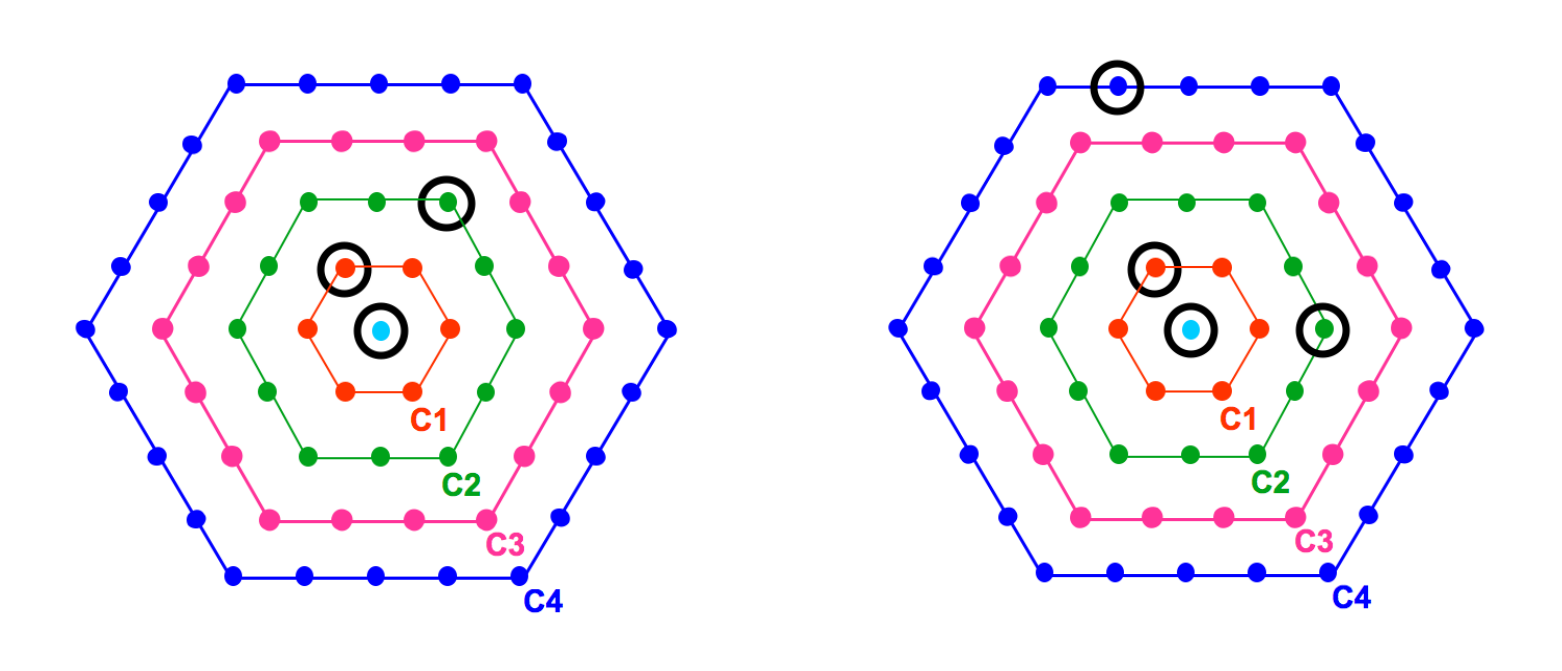
\includegraphics[width=\textwidth]{thesis_figures/Setup/T3_config.png}
%   \caption{Example of two possible T3 configurations. Left: Taken from~\cite{PierreAuger:2010zof}}
%   \label{fig:T3_config}
% \end{figure}

\begin{figure}[t!]
  \centering
  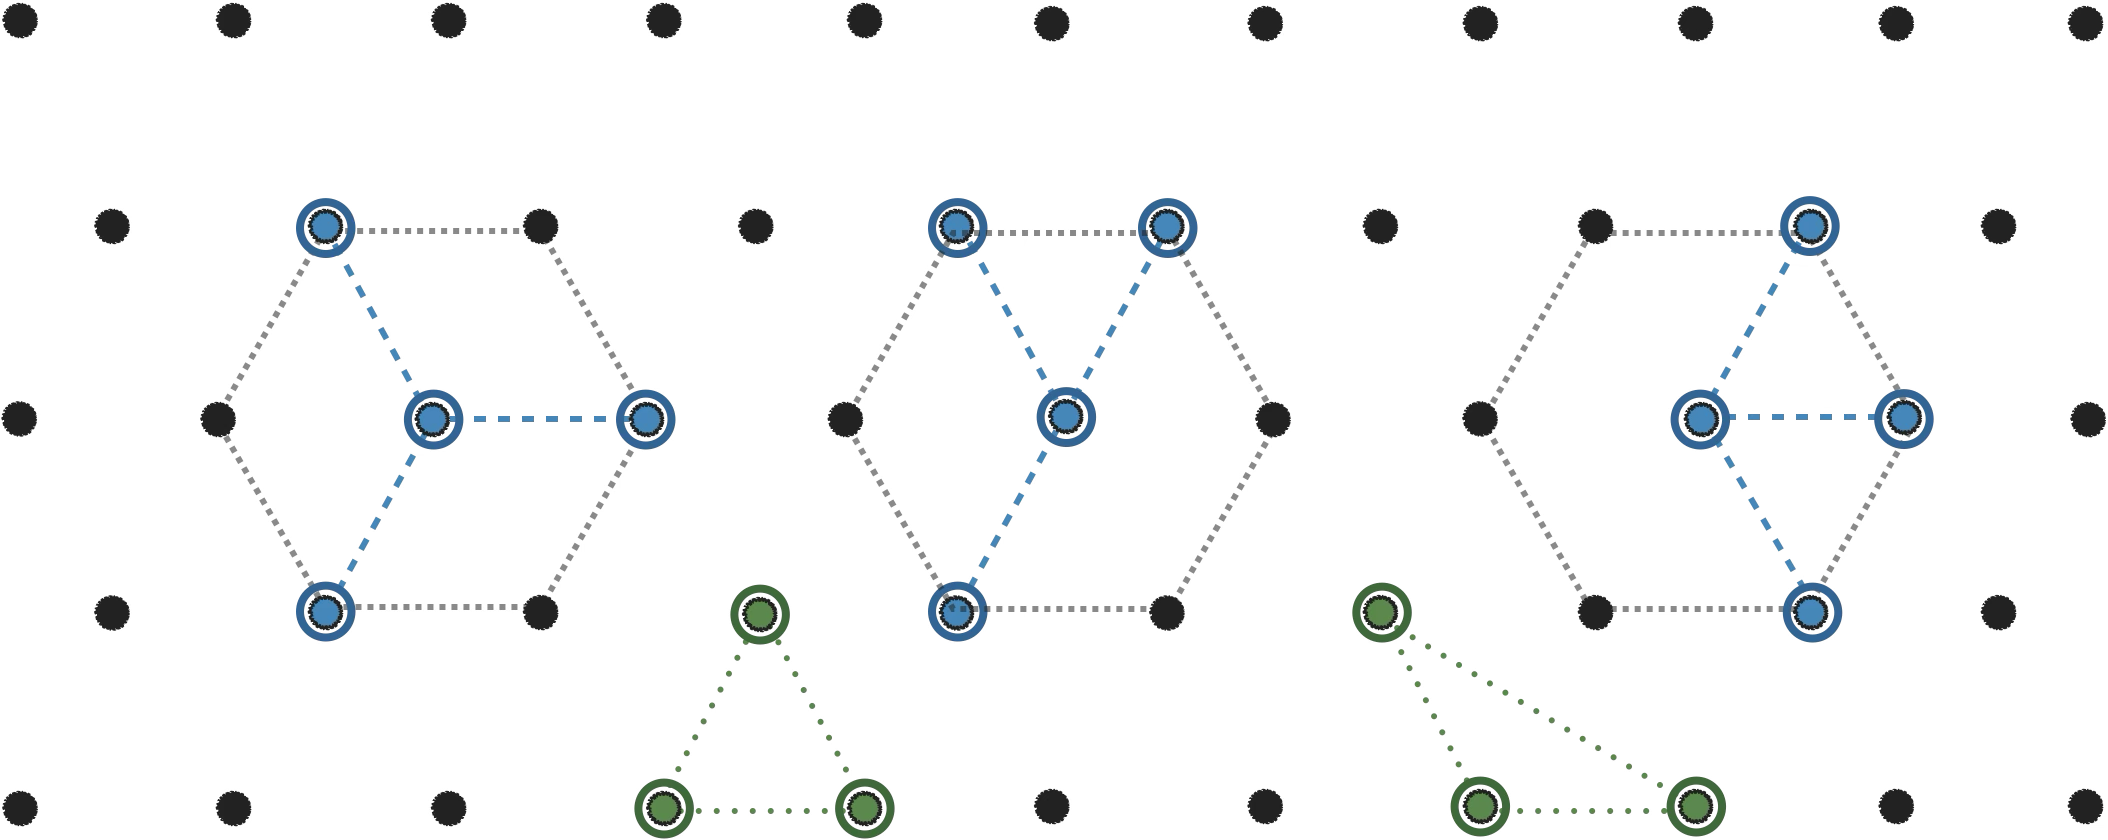
\includegraphics[width=0.75\textwidth]{thesis_figures/Setup/T4_modes.png}
  \caption{Different possible minimal T4 configurations. In blue are the three possible minimal 4C$_1$ configurations while in green are the two possible minimal 3ToT configurations}
  \label{fig:T4_config}
\end{figure}



The next two triggers T4 and T5 are used to improve the data quality. Unlike T1-T3 these are implemented offline. Both check for the geometry and the timing compatibility to select showers in the T3 events. The T4 trigger uses either of the two different criteria to select showers. The first is the requirement of a 3-ToT compact configuration i.e. three nearby stations satisfying the T2-ToT condition in triangular patterns shown in green in Fig.~\ref{fig:T4_config}. The second criterion, 4C1 requires the main triggered station to have at least three triggered tanks out of its six first neighbours as shown in blue in Fig.~\ref{fig:T4_config}. Both the criteria work in collaboration with each other, 3ToT configuration has a selection efficiency of $\sim$99\% for showers below $60^{\circ}$ and the 4C1 configuration helps to recover the rest $\sim$1\% showers lost below $60^{\circ}$ and also selects low energy events above $60^{\circ}$. This trigger is not used for the neutrino analysis.

The T5 fiducial triggers help improve the quality of the showers selected, especially for an accurate energy and angular reconstruction. The trigger ensures the selection of showers that are well contained in the detector array to avoid miss-reconstruction of the core. There are two severity levels for the triggers called 6T5 and 5T5 as shown in fig.~\ref{fig:T5_config}. The former requires all six stations in the first crown around the station with the highest signal to be functional while the latter only requires five. The 6T5 condition helps negate the showers that might fall at any hole in the detector array. These holes can be due to natural obstacles or non-functional tanks. Since 6T5 also improves the angular resolution and improves the overall quality of the selected showers this criterion is used in the search for neutrinos, especially for angles below $75^{\circ}$. Above $75^{\circ}$ since most of the events expected are elongated along a single line the fulfilment of the T5 criteria is very difficult, thus this trigger is not used. 

\section{AugerPrime}
\label{sec:Aug_prime}

AugerPrime~\cite{ANASTASI2022167497} also called Auger Phase 2,  is the ongoing upgrade of the Pierre Auger Observatory to improve its sensitivity and detection capabilities. The upgrade aims to both improve the already present detector systems and also plans to add new components to the observatory. One of the key aims of the \textit{AugerPrime} upgrade is to improve the estimation of the primary CR mass measured by the SD. This is done by the installation of plastic scintillators, \textit{Surface Scintillator Detectors} (SSDs)~\cite{Cataldi:2021uwd} on top of the WCD tanks. The differing responses of WCDs and the SSDs to the electromagnetic and muonic components help enhance the overall mass sensitivity of the detector for vertical showers. The upgrade also replaces the SD electronics (\textit{unified board} and SD front-end board) with the \textit{\acrlong{UUB}} (\acrshort{UUB})~\cite{PierreAuger:2021nnx} and adds a \textit{small} PMT (sPMT)~\cite{PierreAuger:2023clx} to the WCD. The UUBs allow for better station level processing power to account for the SSD and also add a faster sampling rate and better timing accuracy for the SD. The sPMT helps increase the dynamic range of the WCD by reducing the saturated signals in the stations closest to the shower axis. The \textit{AugerPrime} upgrade also includes the deployment of plastic scintillators beneath the WCD tanks, the \acrshort{UMD}~\cite{AbdulHalim:2023ZF} as an extension of AMIGA~\cite{PierreAuger:2021fhj} across the SD-750 and SD-433 sub arrays. The UMD is sensitive to the penetrating muon component of the EAS is very useful for extending the lower energy detection range of the observatory and can also help in photon searches~\cite{PierreAuger:2023nkh}. Deployment of radio antennas on top of each WCD to form \textit{\acrlong{RD}}~\cite{Horandel:2023XL} is also a part of \textit{AugerPrime}. This will allow for the measurement of the radio component of the EAS which originates primarily from the electromagnetic component. Such a measurement especially at very inclined zenith angles will allow for an improved mass estimation even for higher zenith angles where the SSD is insensitive. Additionally, increasing the duty cycle of the FD by operating the telescopes during higher night sky brightness periods with reduced PMT gain is also a part of the upgrade. 

In the context of this thesis, the data from the ongoing upgrade and the preceding test array were not used. However, it is important to mention that the higher sampling rate available with the UUBs and the addition of RD could offer a way to improve the current neutrino analysis. The higher sampling rate could help in reducing the effect of the background muons especially at lower zenith angles ($\sim 60^{\circ}$) whereas the RD in conjunction with WCD could help improve the neutrino detection efficiency for higher zenith angles ($\gtrsim 75^{\circ}$) by improving the T3 efficiency. Also, a general increase in the statistics and continued data taking till the 2030s will help enhance the limits in case of non-detection of cosmogenic neutrinos which have further important implications for the CR spectrum especially for the cutoff as discussed before. The upgrade will also help improve the multi-messenger astronomy capabilities of the observatory. 

\begin{figure}[t!]
  \centering
  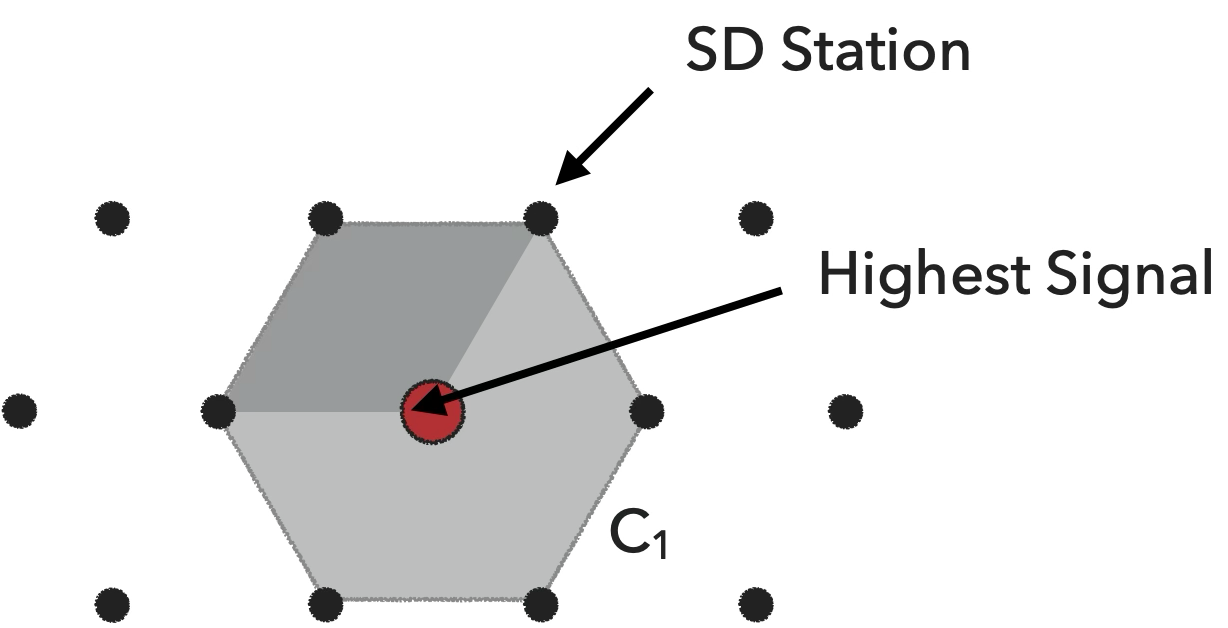
\includegraphics[width=0.5\textwidth]{thesis_figures/Setup/T5_modes.png}
  \caption{Two T5 configurations. The dark shaded hexagon represents the 5T5 condition while the entire shaded hexagons represents the 6T5 hexagon}
  \label{fig:T5_config}
\end{figure}

\section{The \texorpdfstring{$\overline{\text{Off}} \underline{\text{line}}$}{} Framework}
\label{sec:Offline}

The $\mathrm{\overline{Off} \underline{line}}$ framework~\cite{Argiro:2007qg,PierreAuger:2023cqe} is the C++ based software developed internally by the Pierre Auger Observatory to reconstruct air showers and perform cosmic ray analysis. It can process and reconstruct both air shower simulation outputs from generators such as CORSIKA~\cite{Heck:1998vt}, Aires~\cite{Sciutto:1999jh} etc. and the data recorded at the observatory. $\mathrm{\overline{Off} \underline{line}}$ aims to standardize basic quantities such as detector response for simulations and important variables inferred from reconstructing an EAS for the entire collaboration. This helps in providing the collaboration with a homogenous backbone to build physics analysis. It also allows for the physics analysis to be stored and implemented within the framework which helps in leading and optimising productivity. The modular design allows it to be constantly updated for the addition of new functionality and detectors. The framework is available internally on GitLab to the entire Collaboration with regularly planned public releases. $\mathrm{\overline{Off} \underline{line}}$ consists of three fundamental constituents as shown in Fig.~\ref{fig:Offline_schematic}. These are summarised below:



\paragraph*{Detector description:}
This part acts as an input and consists of information about the individual detector systems of the Pierre Auger Observatory. The information is available to the data processing modules as needed but cannot be modified. The static information such as the layout of the detector is stored in XML files whereas the time dependent information such as atmospheric conditions, hardware changes, calibration information etc. is stored in MySQL databases. For real events this allows for an almost perfect duplication of the conditions and for simulations it offers a vast range of available detector configurations.  

\begin{figure}[t!]
  \centering
  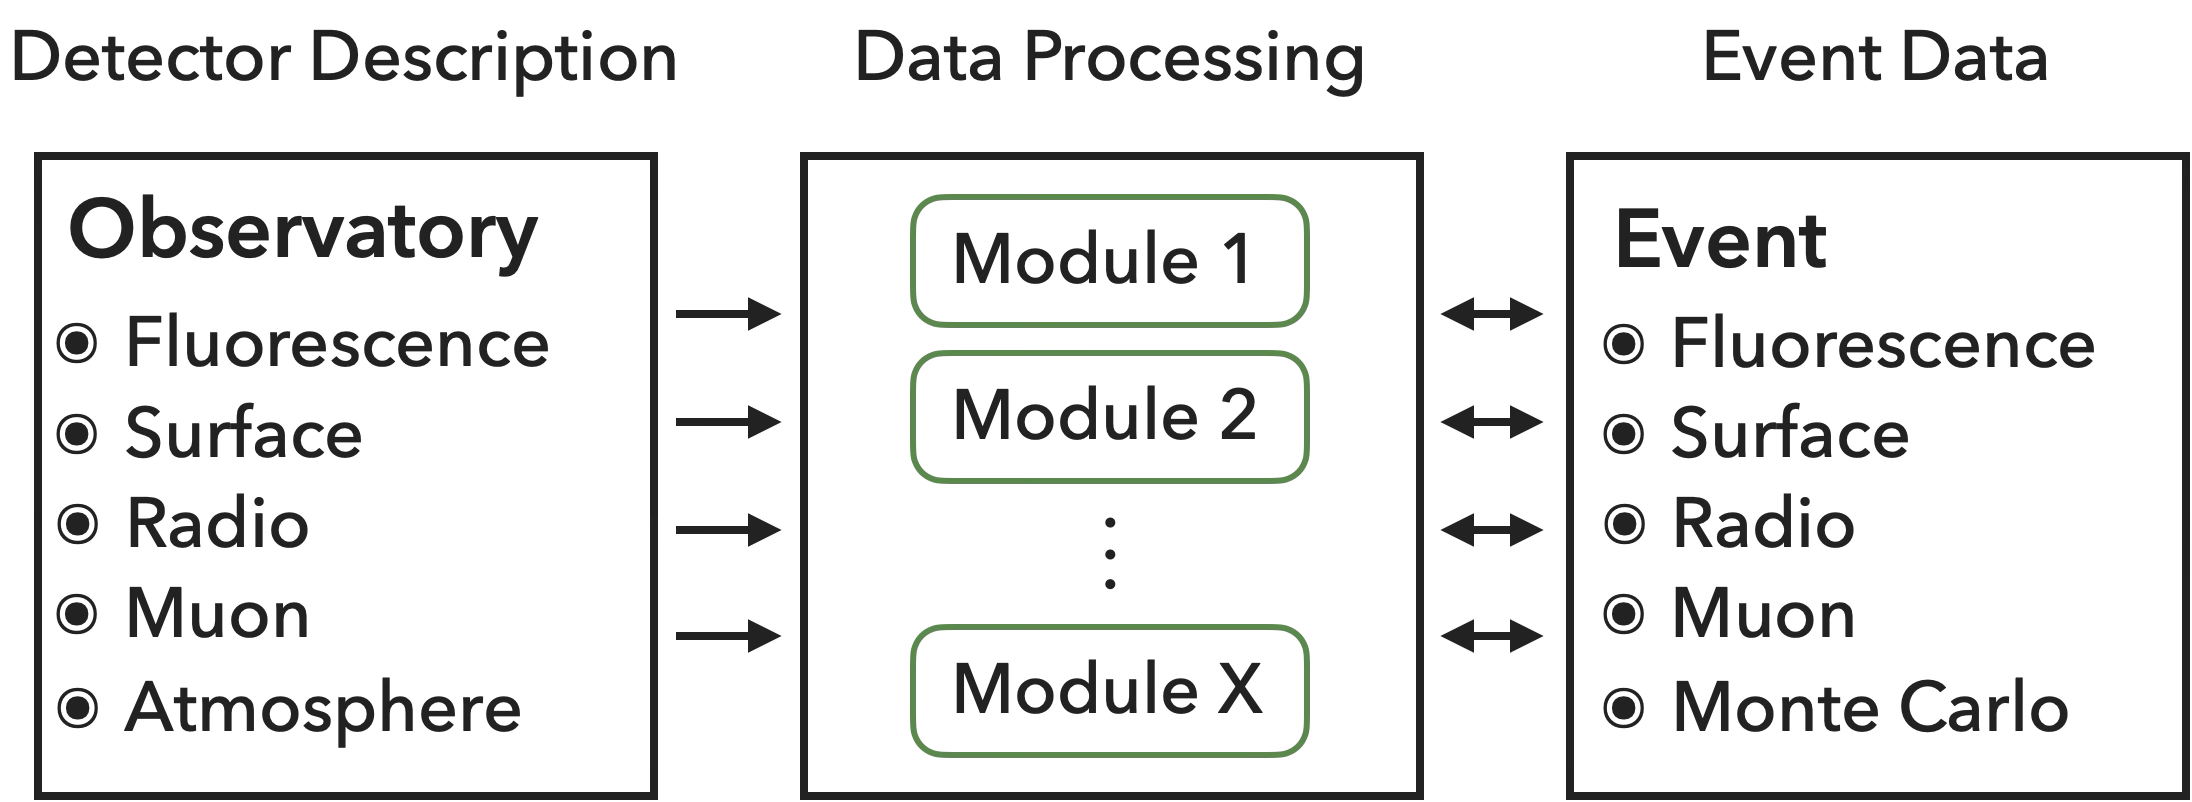
\includegraphics[width=0.75\textwidth]{thesis_figures/Setup/Offline_schematic.png}
  \caption{An Overview of the general structure of $\mathrm{\overline{Off}\underline{line}}$framework. Modified from ~\cite{Argiro:2007qg} }
  \label{fig:Offline_schematic}
\end{figure}

\paragraph*{Event data:}
This part is used to store the important event variables required by modules or the end physics analysis. This includes basic detector level information such as measured or reconstructed signal traces, trigger information etc. to reconstructed variables such as energy, direction or $X_{\text{max}}$. The information is transferred to the data processing modules based on the use case. For a simulation, the event information is first provided to the modules to generate the detector response which is then further reconstructed. In such cases true \gls{MC} values, detector response and the reconstructed quantities are all stored in the event data. Whereas, for real recorded data since the detector response is already present only the reconstruction is performed by the data processing modules. Event data acts as both an input and output for the data processing component of the framework.

\paragraph*{Data processing:}
The type of task performed by the $\mathrm{\overline{Off}\underline{line}}$ is controlled using the data processing components. The different tasks are implemented using individual modules where each module is a self-contained algorithm with the ability to read the detector description. The modules can also read and write event data. Since the modules do not interact with each other they can be easily updated and new modules can be used in an analysis in a plug and play fashion. The different modules can be implemented sequentially in a chosen order based on the analysis. This is controlled via an XML file called Modulesequence.xml. The modules also have adjustable parameters which can either be controlled using individual XML steering files of each module or using a central XML file called bootstrap.xml. There are various standard pre-defined sets of module sequences and bootstraps available in the $\mathrm{\overline{Off}\underline{line}}$ framework which can be directly used without any alterations. For this analysis, one standard reconstruction SdDglNeutrinoReconstruction was tweaked to perform a neutrino search with MoPS and ToTd. Two new reconstruction modules SdDghNeutrinoReconstruction and SdNeutrinoSimulation based on previously done analyses were also adapted and added to the $\mathrm{\overline{Off}\underline{line}}$ framework. The exact modules used in the different neutrino analyses and a description of their functionality are mentioned in the following chapters.

\subsection{Advanced Data Summary Tree}
\label{sec:ADST}
\Glspl{ADST} are ROOT~\cite{Brun:1997pa} based file structures developed internally within the Pierre Auger Collaboration to store the output of the reconstruction. Additionally, it can also be used to store low level information such as detector description, calibration information and also the configuration of the $\mathrm{\overline{Off}\underline{line}}$ framework used to produce the ADST. ADSTs can be used to browse through individual events via the Eventbrowser and carry out higher level physics analysis. Since the structure is based on ROOT ADSTs can be read through different programming languages. In the context of this analysis the ADSTs are interfaced within C++ directly and in python using modules such as Python Instrumentation Kit~\cite{HDembinski_pyik} and uproot~\cite{Pivarski2024-za} in Python. 


%If I want to center something to make a point
% \textbf{Invisible Mode:}
% $A'\rightarrow \chi \overline{\chi}$ signature:
% \begin{flalign*}
%   Beam(p\simeq 100~\text{GeV}),\\
%   E_{ECAL+PS}(< 100~\text{GeV}),\\
%   V_2(< E^{th}_{V}\simeq 1~\text{MIP}),\\
%   E_{HCAL}(< E^{th}_{HCAL}\simeq 1~\text{GeV}).
% \end{flalign*}








%%% Local Variables:
%%% mode: latex
%%% TeX-master: "mythesis"
%%% End:
